%\documentclass[10pt,a4paper]{article}
\documentclass[9pt]{extarticle}
\usepackage[a4paper,top=0.79in,left=0.79in,bottom=0.79in,right=0.79in]{geometry} % A4 paper margins in LibreOffice
\usepackage{hyperref}
\usepackage{amsmath}
\usepackage{amsfonts}
\usepackage{mathrsfs}
\usepackage{bm}
\usepackage{bbm}
\usepackage{stmaryrd}
\usepackage{algorithm}
\usepackage{algorithmic}
\usepackage[sc]{mathpazo}
\linespread{1.05}         % Palladio needs more leading (space between lines)
\usepackage[T1]{fontenc}
\usepackage{subcaption}  % sub-figures
\usepackage{graphicx}
\graphicspath{{fig/}} % Location of the graphics files

\DeclareMathOperator*{\argmin}{argmin}
\DeclareMathOperator*{\argmax}{argmax}
\newcommand{\eat}[1]{}
\setlength{\columnsep}{1.5em} % spacing between columns

\title{The Trajectory Recommendation Problem}

\author{}

\date{}

\begin{document}

\maketitle

\newcommand{\given}{\mid}
\newcommand{\llb}{\llbracket}
\newcommand{\rrb}{\rrbracket}


%\documentclass[10pt,a4paper]{article}
%\documentclass[twocolumn,10pt,a4paper]{article}
%\documentclass[twocolumn,a4wide,9pt]{extarticle}
\documentclass[9pt]{extarticle}
\usepackage[a4paper,top=0.85in,left=0.75in,bottom=1in,right=0.52in]{geometry} % A4 paper margins
%\usepackage[a4paper,top=0.75in,left=0.1in,bottom=0.9in,right=0.1in]{geometry} % A4 paper margins
\usepackage{hyperref}
\usepackage{amsmath}
\usepackage{amsfonts}
\usepackage{mathrsfs}
\usepackage{bm}
\usepackage{bbm}
\usepackage{algorithm}
\usepackage{algorithmic}
\usepackage[sc]{mathpazo}
\linespread{1.05}         % Palladio needs more leading (space between lines)
\usepackage[T1]{fontenc}

\DeclareMathOperator*{\argmin}{argmin}
\DeclareMathOperator*{\argmax}{argmax}
\newcommand{\eat}[1]{}
\setlength{\columnsep}{1.5em} % spacing between columns

\title{The Trajectory Recommendation Problem}

\author{Dawei Chen}

\date{\today}

\begin{document}

\maketitle


\section{Problem formulation}
\label{sec:formulation}

Given a set of points of interest (POI) $\mathcal{P}$ and a trajectory query $\mathbf{x} = (s, K)$,
where $s \in \mathcal{P}$ is the desired start POI and $K$ is the number of POIs in the desired trajectory (including the start location $s$).
We want to recommend a sequence of POIs $\mathbf{y}^*$ that maximises utility, i.e., for a suitable function $f(\cdot,\cdot)$,
\begin{equation*}
\mathbf{y}^* = \argmax_{\mathbf{y}}~f(\mathbf{x}, \mathbf{y}),
\end{equation*}
where $\mathbf{y} = (y_1 = s,~ y_2, \dots, y_K)$ is a trajectory with $K$ POIs, $y_k \in \mathcal{P},~ k=1,\dots,K$, and $y_j \ne y_k$ if $j \ne k$.

On the other hand, we can constrain the desired trajectory with a total time budget $T$ instead of the number of POIs.
In this case, the number of POIs $K$ can be treated as a \emph{hidden} variable, with additional constraint $\sum_{k=1}^K t_k \le T$ 
where $t_k$ is the time spent at POI $y_k$.



\subsection{Related problems}
\label{sec:related}

This problem is related to automatic playlist generation, 
where we recommend a sequence of songs given a specified song (a.k.a. the seed) and the number of new songs.
Formally, given a library of songs and a query $\mathbf{x} = (s, K)$, where $s$ is the seed and $K$ is the number of songs in playlist,
we produce a list with $K$ songs (without duplication) by maximising the likelihood~\cite{chen2012playlist},
\begin{equation*}
%\max_{(y_1,\dots,y_K)} \prod_{k=2}^K \mathbb{P}(y_{k-1} \mid y_k),~ y_1 = s ~\text{and}~ y_j \ne y_k,~ j \ne k.
\mathbf{y}^* = \argmax_{\mathbf{y}} \mathbb{P}(\mathbf{y} \mid \mathbf{x}),~ \mathbf{y} = (y_1=s,\dots,y_K) ~\text{and}~ y_j \ne y_k ~\text{if}~ j \ne k.
\end{equation*}

Another similar problem is choosing a small set of photos from a large photo library and compiling them into a slideshow or movie.



\section{Proposed methods}
\label{sec:methods}

In general, there are two approaches to solve this problem,
\begin{enumerate}
\item \emph{Scoring POIs} (independently), and then pick the $K-1$ highest scored POIs from $\mathcal{P} \setminus s$,
\item \emph{Scoring trajectories}, and then pick the highest scored trajectory with respect to query $\mathbf{x}$.
\end{enumerate}

In this section, we briefly describe a variety of methods that following these two approaches.
Suppose the training set contains $N$ trajectories 
$\{ \mathbf{x}^{(i)}, \mathbf{y}^{(i)} \}_{i=1}^N$,
where $\mathbf{y}^{(i)}$ is the $i$-th trajectory and $\mathbf{x}^{(i)} = (y_1,~ \mid \mathbf{y}^{(i)} \mid)$ is the query 
with respect to trajectory $\mathbf{y}^{(i)}$.



\subsection{POI scoring}
\label{sec:scoring_point}

We have a POI scoring function $S: \mathcal{X} \to \mathbb{R}^{\mid \mathcal{P} \mid}$, 
and the target trajectory is produced by sorting all POIs in descending order according to their scores 
$S(p \mid \mathbf{x}),~ \forall p \in \mathcal{P}$,
then picking the top $K-1$ from $\mathcal{P} \setminus s$.

First, we construct POI feature vectors $\Psi$ and labels $R$ for trajectories in training set, 
\begin{align*}
\Psi &= \left( \Psi(\mathbf{x}^{(i)}, p) \right)_{i=1,\dots,N,~p \in \mathcal{P}} = \left( \Psi_p^i \right)_{i,p}
        \in \mathbb{R}^{(N \cdot \mid \mathcal{P} \mid) \times D}, \\
   R &= \left( r(\mathbf{y}^{(i)}, p \right)_{i=1,\dots,N,~p \in \mathcal{P}} = \left(r_p^i \right)_{i,p}
        \in \mathbb{R}^{(N \cdot \mid \mathcal{P} \mid) \times 1},
\end{align*}
where $D$ is the dimension of feature vector and label $r(\mathbf{y}, p)$ is related to the location POI $p$ in trajectory $\mathbf{y}$,
\begin{equation*}
r(\mathbf{y}, p) = \sum_{j=1}^{\mid \mathbf{y} \mid} (\mid \mathcal{P} \mid - j + 1) \cdot \mathbbm{1}(y_j = p),
\end{equation*}
here $\mathbbm{1}(\cdot)$ is the indicator function, and the $j$-th POI in $\mathbf{y}$ will be scored $\mid \mathcal{P} \mid - j + 1$, 
any POI that does not appear in $\mathbf{y}$ will be scored $0$.
We can also normalise these scores, i.e., $\bar{r}(\mathbf{y}, p) = \frac{1}{\mid \mathcal{P} \mid} r(\mathbf{y}, p)$.


\subsubsection{Occurrence prediction}
\label{sec:logistic}

To begin with, we can simply ignore the order of POIs in a trajectory and just model the occurrence of a POI.
Formally, we construct binary labels
\begin{equation*}
l_p^i = \begin{cases}
+1,~p \in \mathbf{y}^{(i)}, \\
-1,~p \notin \mathbf{y}^{(i)}.
\end{cases}
\end{equation*}
and train a logistic regression model 
%\begin{flalign*} % full-length alignment (align left), note the double-& at the end of equation
%\textsc{\underline{objective}} \hspace{2em} 
\begin{equation*}
\min_{\mathbf{w}} \frac{1}{2} \mathbf{w}^\top \mathbf{w} + 
C \sum_{i=1}^N \sum_{p \in \mathcal{P}} \log \left(1 + \exp \left(- l_p^i \cdot \mathbf{w}_p^\top \Psi_p^i \right) \right), %&&
\end{equation*}
%\end{flalign*}
where $\mathbf{w}$ is an ensemble of all POI specific parameters $\mathbf{w}_p, p \in \mathcal{P}$ and $C>0$ is a regularisation constant.
We can also share parameters between POIs by assuming $\mathbf{w}_p = \mathbf{u} + \mathbf{v}_p$.

The score of POI $p$ is the probability of $p$ occurring in trajectory $\mathbf{y}$ (w.r.t. query $\mathbf{x}$)
\begin{equation*}
S(p \mid \mathbf{x})
= \mathbb{P}(p \in \mathbf{y} \mid \mathbf{x}; \mathbf{w})
= \mathbb{P}(r(\mathbf{y}, p) > 0 \mid \mathbf{x}; \mathbf{w})
= \sigma \left( \mathbf{w}_p^\top \Psi(\mathbf{x}, p) \right),
\end{equation*}
where $\sigma(z) = \frac{1}{1+\exp({-z})}$ is the logistic function.



\subsubsection{Direct rank prediction}
\label{sec:linear}

On the other hand, we can directly model the location/rank of a POI in a trajectory.
Formally, we train a linear regression model to minimise the squared loss $\|r_p^i - \hat{r}_p^i \|_2^2$, 
where the predicted rank $\hat{r}_p^i = \mathbf{w}_p^\top \Psi_p^i$,
\begin{equation*}
\min_{\mathbf{w}} \frac{1}{2} \mathbf{w}^\top \mathbf{w} + C \sum_{i=1}^N \sum_{p \in \mathcal{P}} \|r_p^i - \mathbf{w}_p^\top \Psi_p^i \|_2^2,
\end{equation*}
where parameter settings are similar to those in Section~\ref{sec:logistic}.

The score of POI $p$ is the expected rank of $p$ given query $\mathbf{x}$ 
\begin{equation*}
S(p \mid \mathbf{x})
= \mathbb{E}(\hat{r}_p \mid \mathbf{x}; \mathbf{w}) 
= \mathbf{w}_p^\top \Psi(\mathbf{x}, p).
\end{equation*}

%To learn the parameters $\mathbf{w}$, we need to solve linear equations $\Psi \cdot \mathbf{w} = R$,
%which is straightforward, i.e., $\mathbf{w} = \Psi^{-1} R$ or $\mathbf{w} = \Psi \backslash R$ by using matrix left division.

We note that when two different trajectories satisfy the same query, the feature vectors for all POIs will be the same (see Section~\ref{sec:feature})
but the labels (i.e., ranks) can be different, which may confuse this model, in this case, the prediction will be the average rank.



\subsubsection{Pairwise ranking}
\label{sec:rank}

Let $\phi(\cdot)$ be a loss function and $l_{p,p'}^i$ be a binary label
\begin{equation*}
l_{p,p'}^i = \begin{cases}
+1,~ \mathbf{y}^{(i)} ~\text{prefers}~ p, \\
-1,~ \mathbf{y}^{(i)} ~\text{prefers}~ p'.
\end{cases}
\end{equation*}
We can learn a ranking model
\begin{equation*}
\min_{\mathbf{w}} \frac{1}{2} \mathbf{w}^\top \mathbf{w} +  
C \sum_{i=1}^N \sum_{p, p' \in \mathcal{P}} \phi \left( l_{p,p'}^i \cdot \mathbf{w}^\top \left( \Psi_p^i - \Psi_{p'}^i \right) \right).
\end{equation*}

There are a number of options for the design of loss function $\phi(\cdot)$,
\begin{itemize}
\item if $\phi(z) = \max(0,~ 1-z)^2$, we are training a rankSVM with linear kernel and L2 loss, and the ranking score 
      \begin{equation*}
      S(p \mid \mathbf{x})= \mathbf{w}^\top \Psi(\mathbf{x}, p);
      \end{equation*}
\item if $\phi(z) = \log(1 + \exp(-z))$, we are training a logistic regression model, and the ranking score
      \begin{equation*}
      S(p \mid \mathbf{x})= \mathbb{P}(p \mid \mathbf{x}; \mathbf{w}) = \sigma \left(\mathbf{w}^\top \Psi(\mathbf{x}, p) \right).
      \end{equation*}
\end{itemize}

Similarly, we have a few options for the design of labels $l_{p,p'}^i$,
\begin{itemize}
\item let $c_p^i$ denotes the number of times POI $p$ was observed in trajectories satisfying query $\mathbf{x}^{(i)}$ (except the start POI), and define
      \begin{equation*}
      l_{p,p'}^i = \begin{cases}
      +1,~ c_p^i > c_{p'}^i, \\
      -1,~ c_p^i < c_{p'}^i.
      \end{cases}
      \end{equation*}
      This definition reflects whether $p$ was occurred more frequently than $p'$ for query $\mathbf{x}^{(i)}$.
\item Furthermore, we can implicitly incorporate the ranking of a POI into the binary labels,
      \begin{equation*}
      l_{p,p'}^i = \begin{cases}
      +1,~ r(\mathbf{y}^{(i)}, p) > r(\mathbf{y}^{(i)}, p'), \\
      -1,~ r(\mathbf{y}^{(i)}, p) < r(\mathbf{y}^{(i)}, p').
      \end{cases}
      \end{equation*}
\end{itemize}



\subsection{Trajectory scoring}
\label{sec:structured}

We can model the dependences between different POIs in a trajectory by employing structured prediction models,
either probabilistic models such as maximum-entropy Markov models (MEMM) and conditional random fields (CRF),
or non-probabilistic model such as structured SVM.
We model the desired trajectory with respect to query $\mathbf{x}$ as a sequence of discrete variables, 
with the first variable being observed, and each variable has $|\mathcal{P}|$ states.
To make a recommendation, we find a trajectory that achieves the highest score
\begin{equation*}
\mathbf{y}^* = \argmax_{\mathbf{y} \in \mathcal{Y}}~ f(\mathbf{x}, \mathbf{y}),
\end{equation*}
where $\mathcal{Y}$ is the set of all possible trajectory with POIs in $\mathcal{P}$ and satisfies query $\mathbf{x}$,
$f(\mathbf{x}, \mathbf{y})$ is a function that scores the compatibility between query $\mathbf{x}$ and a specific trajectory $\mathbf{y}$.



\subsubsection{Maximum-entropy Markov models}
\label{sec:memm}

For MEMM, the compatibility function $f(\mathbf{x}, \mathbf{y})$ is the probability of trajectory $\mathbf{y}$ given query $\mathbf{x}$,
\begin{equation*}
f(\mathbf{x}, \mathbf{y}) = \mathbb{P}(\mathbf{y} \mid \mathbf{x}; \mathbf{w}) 
                          = \prod_{j=2}^{\mid \mathbf{y} \mid}~
                            \frac{\exp \left(\mathbf{w}^\top \Psi_j(\mathbf{x}, y_{j-1}, y_j) \right)}
                                 {\sum_{y' \in \mathcal{P}} \exp \left(\mathbf{w}_j^\top \Psi_j(\mathbf{x}, y_{j-1}, y') \right)}.
\end{equation*}

The negative log-likelihood is 
\begin{equation*}
\ell(\mathbf{w}) = -\sum_{i=1}^N \log \mathbb{P}(\mathbf{y}^{(i)} \mid \mathbf{x}^{(i)}; \mathbf{w}) \\
                 = -\sum_{i=1}^N \sum_{j=2}^{\mid \mathbf{y}^{(i)} \mid} 
                    \mathbf{w}^\top \Psi_j(\mathbf{x}^{(i)}, y_{j-1}^{(i)}, y_j^{(i)}) +
                    \sum_{i=1}^N \sum_{j=2}^{\mid \mathbf{y}^{(i)} \mid} 
                    \log \sum_{y' \in \mathcal{P}} \exp \left(\mathbf{w}_j^\top \Psi_j(\mathbf{x}^{(i)}, y_{j-1}^{(i)}, y') \right).
\end{equation*}

To learn the parameters, we minimise the negative log-likelihood with L2 regularisation (maximum likelihood estimation (MLE))
\begin{equation*}
\min_{\mathbf{w}} \frac{1}{2} \mathbf{w}^\top \mathbf{w} + C \ell(\mathbf{w}).
\end{equation*}


\subsubsection{Conditional random fields}
\label{sec:crf}

For linear chain CRF, the compatibility function $f(\mathbf{x}, \mathbf{y})$ is also the probability of trajectory $\mathbf{y}$ given query $\mathbf{x}$,
\begin{equation*}
f(\mathbf{x}, \mathbf{y}) = \mathbb{P}(\mathbf{y} \mid \mathbf{x}; \mathbf{w}) 
= \frac{\exp \left( \mathbf{w}^\top \Psi(\mathbf{x}, \mathbf{y}) \right)}
       {\sum_{\mathbf{y}'} \exp \left( \mathbf{w}^\top \Psi(\mathbf{x}, \mathbf{y}') \right)}
= \frac{\prod_{j=2}^{\mid \mathbf{y} \mid} \exp \left( \mathbf{w}^\top \Psi_j(\mathbf{x}, y_{j-1}, y_j) \right)}
       {\sum_{\mathbf{y}'} \prod_{j=2}^{\mid \mathbf{y}' \mid} \exp \left( \mathbf{w}^\top \Psi_j(\mathbf{x}, y_{j-1}', y_j') \right)},
\end{equation*}
assuming decomposition and parameter tying
\begin{equation*}
\mathbf{w}^\top \Psi(\mathbf{x}, \mathbf{y}) = \sum_{j=2}^{\mid \mathbf{y} \mid} \mathbf{w}^\top \Psi_j(\mathbf{x}, y_{j-1}, y_j).
\end{equation*}

The negative log-likelihood is 
\begin{equation*}
\ell(\mathbf{w}) 
= -\sum_{i=1}^N \log \mathbb{P}(\mathbf{y}^{(i)} \mid \mathbf{x}^{(i)}; \mathbf{w})
= -\sum_{i=1}^N \sum_{j=2}^{\mid \mathbf{y}^{(i)} \mid} \mathbf{w}^\top \Psi_j(\mathbf{x}^{(i)}, y_{j-1}^{(i)}, y_j^{(i)}) +
   \sum_{i=1}^N \log \sum_{\mathbf{y}'} \prod_{j=2}^{\mid \mathbf{y}' \mid} \exp \left( \mathbf{w}^\top \Psi_j(\mathbf{x}^{(i)}, y_{j-1}', y_j') \right).
\end{equation*}

To learn the parameters, we minimise the negative log-likelihood with L2 regularisation (MLE)
\begin{equation*}
\min_{\mathbf{w}} \frac{1}{2} \mathbf{w}^\top \mathbf{w} + C \ell(\mathbf{w}).
\end{equation*}



\subsubsection{Structured SVM}
\label{sec:ssvm}

For structured SVM, the compatibility function $f(\mathbf{x}, \mathbf{y})$ is this linear form,
\begin{equation*}
f(\mathbf{x}, \mathbf{y}) = \mathbf{w}^\top \Psi(\mathbf{x}, \mathbf{y}),
\end{equation*}
where the $\Psi(\mathbf{x}, \mathbf{y})$ is a \emph{joint feature map} 
which captures features extracted from both query $\mathbf{x}$ and trajectory $\mathbf{y}$.

The design of joint feature $\Psi(\cdot)$ is problem specific, 
in the setting of trajectory recommendation,
assuming decomposition and parameter tying, we have
\begin{equation*}
\label{eq:jointfeature}
\mathbf{w}^\top \Psi(\mathbf{x}, \mathbf{y}) = \sum_{j=2}^{\mid \mathbf{y} \mid} 
                                               \left( \mathbf{w}_1^\top \Psi_j(\mathbf{x}, y_j) + 
                                                      \mathbf{w}_2^\top \Psi_{j-1, j}(\mathbf{x}, y_{j-1}, y_j) \right),
\end{equation*}
where $\mathbf{w}_1$ and $\mathbf{w}_2$ are parameter vectors,
$\Psi_j$ is a feature vector of POI $y_j$ with respect to query $\mathbf{x}$ (Table~\ref{tab:poifeature}),
$\Psi_{j-1,j}$ is a pairwise feature vector that captures the affinity of transition from POI $y_{j-1}$ to POI $y_j$ and
here we use the transition probabilities between individual POI properties as described in Table~\ref{tab:tranfeature}.
This joint feature design shares parameters among POIs/transitions in a trajectory.

To learn the parameters, we train the structured SVM by optimising a quadratic program (QP),
\begin{equation}
\label{eq:nslackform}
\begin{aligned}
\min_{\mathbf{w}, ~\bm{\xi} \ge 0} ~& \frac{1}{2} \mathbf{w}^\top \mathbf{w} + \frac{C}{n} \sum_{i=1}^n \xi_i \\
s.t.~~ ~& \mathbf{w}^\top \Psi(\mathbf{x}^{(i)}, \mathbf{y}^{(i)}) - \mathbf{w}^\top \Psi(\mathbf{x}^{(i)}, \bar{\mathbf{y}}) \ge 
       \Delta(\mathbf{y}^{(i)}, \bar{\mathbf{y}}) - \xi_i, ~\forall i
\end{aligned}
\end{equation}
where $\mathbf{w} = [\mathbf{w}_1, \mathbf{w}_2]^\top$ is the parameter vector, $C > 0$ is a regularisation constant, 
and $\Delta(\mathbf{y}, \bar{\mathbf{y}})$ is a discrepancy function that measures the loss 
for prediction $\bar{\mathbf{y}}$ given ground truth $\mathbf{y}$, and $\xi_i$
is a slack variable that represents the \emph{hinge loss} associated with the prediction for the $i$-th example~\cite{tsochantaridis2005large},
\begin{equation*}
\label{eq:nslackloss}
\xi_i = \max \left( 0,~ 
        \max_{\bar{\mathbf{y}} \in \mathcal{Y}} 
        \left\{ \Delta(\mathbf{y}_i, \bar{\mathbf{y}}) + \mathbf{w}^\top \Psi(\mathbf{x}^{(i)}, \bar{\mathbf{y}}) \right\} -
        \mathbf{w}^\top \Psi(\mathbf{x}^{(i)}, \mathbf{y}^{(i)}) \right).
\end{equation*}
%This formulation is called "$n$-slack" as we have one slack variable for each example in training set.

We can rewrite the constraint of problem (\ref{eq:nslackform}) as
\begin{equation*}
\mathbf{w}^\top \Psi(\mathbf{x}^{(i)}, \mathbf{y}^{(i)}) + \xi_i \ge
          \max_{\bar{\mathbf{y}} \in \mathcal{Y}} 
          \left\{\mathbf{w}^\top \Psi(\mathbf{x}^{(i)}, \bar{\mathbf{y}}) + \Delta(\mathbf{y}^{(i)}, \bar{\mathbf{y}}) \right\},~ \forall i.
\end{equation*}
where the right hand side is the \emph{loss-augmented inference}.

To solve problem (\ref{eq:nslackform}), one option is simply enumerating all constraints, feeding the problem into a standard QP solver.
However, this approach is impractical as there is a constraint for every possible label $\bar{\mathbf{y}}$.
Instead, a cutting-plane algorithm is employed which repeatedly solves QP (\ref{eq:nslackform}) with respect to different set of constraints, 
and each iteration solves the loss-augmented inference and generates a new constraint that helps shrink the feasible region of the problem, 
until a specified precision $\varepsilon$ is achieved~\cite{joachims2009predicting}.

The loss-augmented inference for trajectory recommendation is equivalent to 
find a maximum weighted loop-less path with exactly $k$ edges in a complete weighted (both nodes and edges) graph, which is NP-hard (need proof).
To solve the loss-augmented inference, we can formulated it as an integer linear program (ILP) and solve it using a ILP solver,
or use lazy constraint generation/cutting plane technique with an LP solver.
Moreover, we can use list Viterbi algorithm~\cite{nill1995list} or 
employ heuristics such as the Christofides algorithm~\cite{christofides1976} when the problem has the triangle inequality property 
(which is indeed for trajectories).


\eat{
\subsection{Other models}
\label{sec:other}
Label ranking model,
Plackett-Luce probabilistic ranking


\section{Evaluation metrics}
\label{sec:evaluation}
F1 score on points
F1 score on pairs
Kendall's tau, all POIs not appeared in trajectory are ranked last (and share the same rank).
}


\begin{table*}[ht]
\caption{Features of POI $p$ with respect to query $(s,k)$}
\label{tab:poifeature}
\centering
\setlength{\tabcolsep}{10pt} % tweak the space between columns
\begin{tabular}{l|l} \hline
\textbf{Feature}  & \textbf{Description} \\ \hline
\texttt{category}               & one-hot encoding of the category of $p$ \\
\texttt{neighbourhood}          & one-hot encoding of the POI cluster that $p$ resides in \\
\texttt{popularity}             & logarithm of POI popularity of $p$ \\
\texttt{nVisit}                 & logarithm of the total number of visit by all users at $p$ \\
\texttt{avgDuration}            & logarithm of the average duration at $p$ \\ \hline
\texttt{trajLen}                & trajectory length $k$, i.e., the number of POIs required \\
\texttt{sameCatStart}           & $1$ if the category of $p$ is the same as that of $s$, $-1$ otherwise \\
\texttt{sameNeighbourhoodStart} & $1$ if $p$ resides in the same POI cluster as $s$, $-1$ otherwise \\
\texttt{distStart}              & distance between $p$ and $s$, calculated using the Haversine formula \\
\texttt{diffPopStart}           & real-valued difference in POI popularity of $p$ from that of $s$ \\
\texttt{diffNVisitStart}        & real-valued difference in the total number of visit at $p$ from that at $s$ \\
\texttt{diffDurationStart}      & real-valued difference in average duration at $p$ from that at $s$ \\
\hline
\end{tabular}
\end{table*}


\section{Features}
\label{sec:feature}

The POI and query specific features we extracted from trajectories are shown in Table~\ref{tab:poifeature},
features that describe the transition preference between different POIs are shown in Table~\ref{tab:tranfeature}.


\begin{table}[ht]
\caption{POI features used to estimate the (feature-wise) transition probabilities}
\label{tab:tranfeature}
\centering
%\setlength{\tabcolsep}{28pt} % tweak the space between columns
\begin{tabular}{l|l} \hline
\textbf{Feature}       & \textbf{Description} \\ \hline
\texttt{category}      & category of POI \\
\texttt{neighbourhood} & the cluster that a POI resides in \\
\texttt{popularity}    & (discretised) popularity of POI \\
\texttt{nVisit}        & (discretised) total number of visit at POI \\
\texttt{avgDuration}   & (discretised) average duration at POI \\ \hline
\end{tabular}
\end{table}



\bibliographystyle{ieeetr}
\bibliography{ref}

\end{document}

\section{Proposed methods}
\label{sec:methods}

In general, there are two approaches to solve this problem,
\begin{enumerate}
\item \emph{Scoring POIs}, and then pick the $K-1$ highest scored POIs from $\mathcal{P} \setminus s$,
\item \emph{Scoring trajectories}, and then pick the highest scored trajectory with respect to query $\mathbf{x}$.
\end{enumerate}

In this section, we briefly describe a variety of methods that following these two approaches.
Suppose the training set contains $N$ trajectories 
$\{ \mathbf{x}^{(i)}, \mathbf{y}^{(i)} \}_{i=1}^N$,
where $\mathbf{y}^{(i)}$ is the $i$-th trajectory and $\mathbf{x}^{(i)} = (y_1^{(i)},~ | \mathbf{y}^{(i)} |)$ is the query 
with respect to trajectory $\mathbf{y}^{(i)}$.



\subsection{Scoring POIs}
\label{sec:scoring_point}

We have a POI scoring function $S: \mathcal{X} \to \mathbb{R}^{| \mathcal{P} |}$, 
and the target trajectory is produced by sorting all POIs in descending order according to their scores 
$S(p | \mathbf{x}),~ \forall p \in \mathcal{P}$,
then picking the top $K-1$ from $\mathcal{P} \setminus s$.

First, we construct POI feature vectors $\Psi$ and labels $R$ for trajectories in training set, 
\begin{align*}
\Psi &= \left( \Psi(\mathbf{x}^{(i)}, p) \right)_{i=1,\dots,N,~p \in \mathcal{P}} = \left( \Psi_p^i \right)_{i,p}
        \in \mathbb{R}^{(N \cdot | \mathcal{P} |) \times D}, \\
   R &= \left( r(\mathbf{y}^{(i)}, p) \right)_{i=1,\dots,N,~p \in \mathcal{P}} = \left(r_p^i \right)_{i,p}
        \in \mathbb{R}^{(N \cdot | \mathcal{P} |) \times 1},
\end{align*}
where $D$ is the dimension of feature vector and label $r(\mathbf{y}, p)$ is computed from the location of POI $p$ in trajectory $\mathbf{y}$,
\begin{equation*}
r(\mathbf{y}, p) = \frac{1}{| \mathcal{P} |} 
                   \sum_{j=1}^{| \mathbf{y} |} (| \mathcal{P} | - j + 1) \cdot \llb y_j = p \rrb,
\end{equation*}
here $\llb \cdot \rrb$ is the indicator function, and the $j$-th POI in $\mathbf{y}$ will be scored $| \mathcal{P} | - j + 1$, 
any POI that does not appear in $\mathbf{y}$ will be scored $0$ ($0$ is an arbitrary choice).



\subsubsection{Occurrence prediction}
\label{sec:logistic}

To begin with, we can simply ignore the order of POIs in a trajectory and just model the occurrence of a POI.
Formally, we construct binary labels
\begin{equation*}
l_p^i = \begin{cases}
+1,~p \in \mathbf{y}^{(i)} \\
-1,~p \notin \mathbf{y}^{(i)}
\end{cases}
\hspace{-1em}
= \begin{cases}
+1,~ r_p^i > 0 \\
-1,~ r_p^i = 0
\end{cases}
\end{equation*}
and train a logistic regression model 
%\begin{flalign*} % full-length alignment (align left), note the double-& at the end of equation
%\textsc{\underline{objective}} \hspace{2em} 
\begin{equation*}
\min_{\mathbf{w}} \frac{1}{2} \mathbf{w}^\top \mathbf{w} + 
%C \sum_{i=1}^N \sum_{p \in \mathcal{P}} \log \left(1 + \exp (- l_p^i \cdot \mathbf{w}_p^\top \Psi_p^i) \right), %&&
C \sum_{i=1}^N \sum_{p \in \mathcal{P}} \phi \left( l_p^i \cdot \mathbf{w}_p^\top \Psi_p^i) \right), %&&
\end{equation*}
%\end{flalign*}
where $\phi(z) = \log(1+\exp(-z))$ is a loss function, $\mathbf{w}$ is an ensemble of all POI specific parameters $\mathbf{w}_p, p \in \mathcal{P}$,
and $C>0$ is a regularisation constant.
We can also share parameters between POIs by assuming $\mathbf{w}_p = \mathbf{u} + \mathbf{v}_p$.

The score of POI $p$ is the probability of $p$ occurring in trajectory $\mathbf{y}$ given query $\mathbf{x}$
\begin{equation*}
S(p \given \mathbf{x})
= \mathbb{P}(p \in \mathbf{y} \given \mathbf{x}; \mathbf{w})
= \mathbb{P}(r(\mathbf{y}, p) > 0 \given \mathbf{x}; \mathbf{w})
= \sigma \left( \mathbf{w}_p^\top \Psi(\mathbf{x}, p) \right),
\end{equation*}
where $\sigma(z) = \frac{1}{1+\exp({-z})}$ is the logistic function.



\subsubsection{POI scoring for each location}
\label{sec:multi}

Furthermore, we can model the probability of POI $p$ at location $k$ given query $\mathbf{x}$.
That is, for each query $\mathbf{x}^{(i)},~ \forall i$, 
we train a $| \mathcal{P} |$-class $K$-label classifier with examples $\{ \mathbf{x}^{(i)}, y_k^{(i)} \}_{k=2}^K$
using the one-versus-rest approach,
\begin{equation*}
\mathbb{P}(y_k = p \given \mathbf{x}) = \frac{\exp \left( \mathbf{w}^\top \Psi(\mathbf{x}, p, k) \right)}
                                           {\sum_{p' \in \mathcal{P}} \exp \left( \mathbf{w}^\top \Psi(\mathbf{x}, p', k) \right)}.
\end{equation*}

The recommendation is simply done by picking the most likely POI for each location $k$ independently,
\begin{equation*}
y_k^* = \argmax_{p \in \mathcal{P}}~ \mathbb{P}(y_k = p \given \mathbf{x}),~ k = 2, \dots, K.
\end{equation*}

This approach can be described by a directed graphical model as shown in Figure~\ref{fig:pgm}(a).



\subsubsection{Direct rank prediction}
\label{sec:linear}

On the other hand, we can directly model the location/rank of a POI in a trajectory.
Formally, we train a linear regression model to minimise the empirical squared loss (with L2 regularisation)
\begin{equation*}
\min_{\mathbf{w}} \frac{1}{2} \mathbf{w}^\top \mathbf{w} + C \sum_{i=1}^N \sum_{p \in \mathcal{P}} \|r_p^i - \hat{r}_p^i \|^2, 
\end{equation*}
where the predicted rank $\hat{r}_p^i = \mathbf{w}_p^\top \Psi_p^i$, 
and parameter settings are similar to those described in Section~\ref{sec:logistic},
and examples with $0$ labels, i.e., $r_p^i = 0$ are ignored in training.

The score of POI $p$ is the expected rank of $p$ given query $\mathbf{x}$ 
\begin{equation*}
S(p \given \mathbf{x})
= \mathbb{E}(\hat{r}_p | \mathbf{x}; \mathbf{w}) 
= \mathbf{w}_p^\top \Psi(\mathbf{x}, p).
\end{equation*}

%To learn the parameters $\mathbf{w}$, we need to solve linear equations $\Psi \cdot \mathbf{w} = R$,
%which is straightforward, i.e., $\mathbf{w} = \Psi^{-1} R$ or $\mathbf{w} = \Psi \backslash R$ by using matrix left division.

We note that when two different trajectories satisfy the same query, the feature vectors (Section~\ref{sec:feature}) for all POIs will be the same 
but the labels (i.e., ranks) can be different, which may confuse this model. In this case, the prediction (by this model) will be the average rank.




\subsubsection{Pairwise ranking}
\label{sec:rank}

Let $\phi(\cdot)$ be a loss function and $l_{p,p'}^i$ be a binary label
\begin{equation*}
l_{p,p'}^i = \begin{cases}
+1,~ \mathbf{y}^{(i)} ~\text{prefers}~ p, \\
-1,~ \mathbf{y}^{(i)} ~\text{prefers}~ p'.
\end{cases}
\end{equation*}
We can learn a ranking model
\begin{equation*}
\min_{\mathbf{w}} \frac{1}{2} \mathbf{w}^\top \mathbf{w} +  
C \sum_{i=1}^N \sum_{p, p' \in \mathcal{P}} \phi \left( l_{p,p'}^i \cdot \mathbf{w}^\top (\Psi_p^i - \Psi_{p'}^i) \right).
\end{equation*}
Due to symmetry, it is necessary to consider only the pairs $(p, p')$ when $l_{p, p'}^i = +1$, which means we can further simplify 
the cost function of the ranking model
\begin{equation*}
\min_{\mathbf{w}} \frac{1}{2} \mathbf{w}^\top \mathbf{w} +  
C \sum_{i=1}^N \sum_{\substack{p, p' \in \mathcal{P} \\ l_{p,p'}^i > 0}} \phi \left(\mathbf{w}^\top (\Psi_p^i - \Psi_{p'}^i) \right).
\end{equation*}

There are a number of options for the design of labels $l_{p,p'}^i$,
\begin{itemize}
\item let $c_p^i$ denotes the number of times POI $p$ was observed in trajectories satisfying query $\mathbf{x}^{(i)}$ (except the start POI), and define
      \begin{equation*}
      l_{p,p'}^i = \begin{cases}
      +1,~ c_p^i > c_{p'}^i, \\
      -1,~ c_p^i < c_{p'}^i.
      \end{cases}
      \end{equation*}
      This definition reflects whether $p$ was occurred more frequently than $p'$ for query $\mathbf{x}^{(i)}$.
      To deal with ties, i.e., $\{(p, p') | c_p^i = c_{p'}^i\}$, we generate both the positive and the negative labels for these examples.
\item Alternatively, we can define
      \begin{equation*}
      l_{p,p'}^i = \begin{cases}
      +1,~ r(\mathbf{y}^{(i)}, p) > r(\mathbf{y}^{(i)}, p'), \\
      -1,~ r(\mathbf{y}^{(i)}, p) < r(\mathbf{y}^{(i)}, p').
      \end{cases}
      \end{equation*}
      There will be no ties when $p \ne p'$ and $p, p' \in \mathbf{y}^{(i)}$, if we remove examples that $r_p^i = 0$.
\end{itemize}


Similarly, we have a few options for the design of loss function $\phi(\cdot)$,
\begin{itemize}
\item if $\phi(z) = \max(0,~ 1-z)^2$, we are training a rankSVM with linear kernel and L2 loss, and the ranking score 
      \begin{equation*}
      S(p \given \mathbf{x})= \mathbf{w}^\top \Psi(\mathbf{x}, p);
      \end{equation*}
      We can train this ranking model by gradient descent. Let $J(\mathbf{w})$ be the cost function that we want to minimise, i.e.,
      \begin{align*}
      J(\mathbf{w})
      &= \frac{1}{2} \mathbf{w}^\top \mathbf{w} +  
         C \sum_{i=1}^N \sum_{\substack{p, p' \in \mathcal{P} \\ l_{p,p'}^i >0}} \phi \left( \mathbf{w}^\top (\Psi_p^i - \Psi_{p'}^i) \right) \\
      &= \frac{1}{2} \mathbf{w}^\top \mathbf{w} + 
         C \sum_{i=1}^N \sum_{\substack{p, p' \in \mathcal{P} \\ l_{p,p'}^i >0}} \max\left(0,~ 1 - \mathbf{w}^\top (\Psi_p^i - \Psi_{p'}^i) \right)^2.
      \end{align*}
      To compute the gradient of the cost function w.r.t. parameters, note that
      \begin{equation*}
      \max(0,~ 1-z)^2 
      = \begin{cases}
        (1-z)^2, & z \le 1 \\
        0,       & z > 1
        \end{cases}
      \end{equation*} 
      and $\lim_{z \to 1} \max(0,~ 1-z)^2 = 0$, which means the loss function is differentiable at $z=1$ and its gradient is
      \begin{equation*}
      \frac{\partial \max(0,~ 1-z)^2}{\partial z} 
      = \begin{cases}
        -2(1-z), & z \le 1 \\
        0,       & z > 1
        \end{cases}
      \end{equation*} 
      As a result, the gradient of the cost function w.r.t. parameters $\mathbf{w}$ is
      \begin{align*}
      \frac{\partial J(\mathbf{w})}{\partial \mathbf{w}} 
      = \mathbf{w} + C \sum_{i=1}^N \sum_{\substack{p, p' \in \mathcal{P} \\ l_{p,p'}^i >0}} g_{p,p'}^i(\mathbf{w})
      \end{align*} 
      where 
      \begin{equation*}
      g_{p,p'}^i(\mathbf{w}) 
      = \begin{cases}
        -2 \cdot (\Psi_p^i - \Psi_{p'}^i) \cdot \left(1 - \mathbf{w}^\top (\Psi_p^i - \Psi_{p'}^i) \right), 
        & \mathbf{w}^\top (\Psi_p^i - \Psi_{p'}^i) \le 1 \\
        0, 
        & \text{otherwise}
        \end{cases}
      \end{equation*}

\item if $\phi(z) = \log(1 + \exp(-z))$, we are training a logistic regression model, and the ranking score
      \begin{equation*}
      S(p \given \mathbf{x})= \mathbb{P}(p \given \mathbf{x}; \mathbf{w}) = \sigma \left(\mathbf{w}^\top \Psi(\mathbf{x}, p) \right).
      \end{equation*}
      We can train this ranking model by gradient descent. The cost function is
      \begin{align*}
      J(\mathbf{w})
      &= \frac{1}{2} \mathbf{w}^\top \mathbf{w} +  
         C \sum_{i=1}^N \sum_{\substack{p, p' \in \mathcal{P} \\ l_{p,p'}^i >0}} \phi \left( \mathbf{w}^\top (\Psi_p^i - \Psi_{p'}^i) \right) \\
      &= \frac{1}{2} \mathbf{w}^\top \mathbf{w} + C \sum_{i=1}^N \sum_{\substack{p, p' \in \mathcal{P} \\ l_{p,p'}^i >0}} 
         \log\left(1 + \exp\left( -\mathbf{w}^\top (\Psi_p^i - \Psi_{p'}^i) \right)\right).
      \end{align*}
      The gradient of the cost function w.r.t. parameters $\mathbf{w}$ is
      \begin{align*}
      \frac{\partial J(\mathbf{w})}{\partial \mathbf{w}} 
      &= \mathbf{w} + C \sum_{i=1}^N \sum_{\substack{p, p' \in \mathcal{P} \\ l_{p,p'}^i >0}}
         \frac{-(\Psi_p^i - \Psi_{p'}^i) \cdot \exp\left( -\mathbf{w}^\top (\Psi_p^i - \Psi_{p'}^i) \right)}
              {1 + \exp\left( -\mathbf{w}^\top (\Psi_p^i - \Psi_{p'}^i) \right)} \\
      &= \mathbf{w} + C \sum_{i=1}^N \sum_{\substack{p, p' \in \mathcal{P} \\ l_{p,p'}^i >0}}
         \frac{-(\Psi_p^i - \Psi_{p'}^i)}{1 + \exp\left( \mathbf{w}^\top (\Psi_p^i - \Psi_{p'}^i) \right)}.
      \end{align*} 
\end{itemize}

      
Compared with the first definition, the second option can implicitly incorporate the rank of a POI into the binary labels.



\subsubsection{Discussion}

We note that the point-wise POI scoring approaches (Section~\ref{sec:logistic} to \ref{sec:linear}) do not consider the inter-dependencies between POIs,
and the pairwise ranking approach (Section~\ref{sec:rank}) only considers the relative order between two individual points,
i.e., modelling each pair independently.



\subsection{Scoring trajectories}
\label{sec:structured}

One approach that captures long-term dependencies is scoring a trajectory as a whole,
that is, we model the dependences between different POIs in a trajectory by employing structured prediction models,
e.g., probabilistic models such as maximum-entropy Markov models (MEMM) and conditional random fields (CRF),
or non-probabilistic model such as structured SVM.

We model the desired trajectory with respect to query $\mathbf{x}$ as a sequence of discrete variables with inter-dependencies,
each variable has $|\mathcal{P}|$ states, and the first variable being observed.
To make a recommendation, we find a trajectory that achieves the highest score
\begin{equation*}
\mathbf{y}^* = \argmax_{\mathbf{y} \in \mathcal{Y}_\mathbf{x}}~ f(\mathbf{x}, \mathbf{y}),
\end{equation*}
%where $\mathcal{Y}_\mathbf{x}$ is the set of all possible trajectories with POIs in $\mathcal{P}$ and satisfying query $\mathbf{x}$,
where $f(\mathbf{x}, \mathbf{y})$ is a function that scores the compatibility between query $\mathbf{x}$ and a specific trajectory $\mathbf{y}$,
and different models described in this section basically employ different formulations of $f(\cdot,\cdot)$. % with respect to different assumptions.


\begin{figure}[t]
    \centering
    \begin{subfigure}[t]{.33\textwidth} % textwidth in figure environment
        \centering
        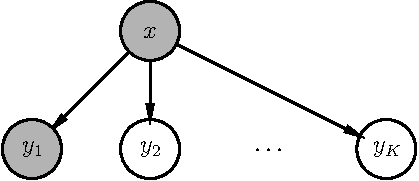
\includegraphics[width=.8\textwidth]{mmclassifier.pdf} % textwidth in subfigure environment
        \caption{Multi-class multi-label classifier}
    \end{subfigure}
    \begin{subfigure}[t]{.33\textwidth}
        \centering
        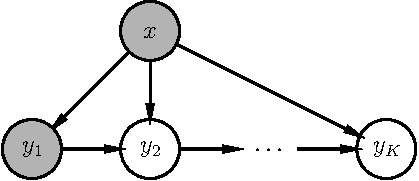
\includegraphics[width=.8\textwidth]{memm.pdf}
        \caption{MEMM}
    \end{subfigure}
    \begin{subfigure}[t]{.33\textwidth}
        \centering
        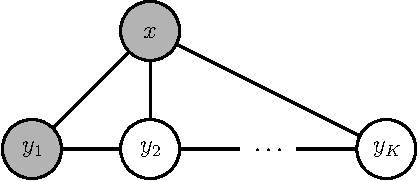
\includegraphics[width=.8\textwidth]{crf.pdf}
        \caption{CRF}
    \end{subfigure}
    \caption{Graphical models for trajectory recommendation.}
    \label{fig:pgm}
\end{figure}


\subsubsection{Maximum-entropy Markov models}
\label{sec:memm}

For MEMM, the compatibility function $f(\mathbf{x}, \mathbf{y})$ is the probability of trajectory $\mathbf{y}$ given query $\mathbf{x} = (s, K)$,
\begin{equation*}
f(\mathbf{x}, \mathbf{y}) 
= \mathbb{P}(\mathbf{y} \given \mathbf{x}; \mathbf{w}) 
= \mathbb{P}(y_1 \given \mathbf{x}; \mathbf{w}) \cdot \prod_{j=2}^K \mathbb{P}(y_j \given y_{j-1}, \mathbf{x}; \mathbf{w})
= 1 \cdot \prod_{j=2}^{K}~
  \frac{\exp \left(\mathbf{w}^\top \Psi_j(\mathbf{x}, y_{j-1}, y_j) \right)}
       {\sum_{y' \in \mathcal{P}} \exp \left(\mathbf{w}^\top \Psi_j(\mathbf{x}, y_{j-1}, y') \right)},
\end{equation*}
where we do local normalisation.

The negative log-likelihood of training set is
\begin{equation*}
\ell(\mathbf{w}) 
= -\sum_{i=1}^N \log \mathbb{P}(\mathbf{y}^{(i)} \given \mathbf{x}^{(i)}; \mathbf{w}) \\
= -\sum_{i=1}^N \sum_{j=2}^{| \mathbf{y}^{(i)} |} 
                \mathbf{w}^\top \Psi_j(\mathbf{x}^{(i)}, y_{j-1}^{(i)}, y_j^{(i)}) +
   \sum_{i=1}^N \sum_{j=2}^{| \mathbf{y}^{(i)} |} 
                \log \sum_{y' \in \mathcal{P}} \exp \left(\mathbf{w}^\top \Psi_j(\mathbf{x}^{(i)}, y_{j-1}^{(i)}, y') \right).
\end{equation*}

To learn the parameters, we maximise the likelihood of training set by minimising its negative log-likelihood (with L2 regularisation)
\begin{equation}
\label{eq:trainmemm}
\min_{\mathbf{w}} \frac{1}{2} \mathbf{w}^\top \mathbf{w} + C \ell(\mathbf{w}).
\end{equation}

A straightforward approach to optimise the above objective is employing gradient descent. 
Let $J(\mathbf{w})$ be the objective (cost function), i.e.,
\begin{align*}
J(\mathbf{w}) 
&= \frac{1}{2} \mathbf{w}^\top \mathbf{w} + C \ell(\mathbf{w}) \\
&= \frac{1}{2} \mathbf{w}^\top \mathbf{w} -
   C \sum_{i=1}^N \sum_{j=2}^{| \mathbf{y}^{(i)} |} \mathbf{w}^\top \Psi_j(\mathbf{x}^{(i)}, y_{j-1}^{(i)}, y_j^{(i)}) +
   C \sum_{i=1}^N \sum_{j=2}^{| \mathbf{y}^{(i)} |} \log \sum_{y' \in \mathcal{P}} 
     \exp \left(\mathbf{w}^\top \Psi_j(\mathbf{x}^{(i)}, y_{j-1}^{(i)}, y') \right).
\end{align*}
The gradient of the cost function w.r.t. parameters $\mathbf{w}$ is
\begin{align*}
\frac{\partial J{\mathbf{w}}}{\partial \mathbf{w}}
&= \mathbf{w} + C \frac{\partial \ell(\mathbf{w})}{\partial \mathbf{w}} \\
&= \mathbf{w} - C \sum_{i=1}^N \sum_{j=2}^{| \mathbf{y}^{(i)} |} \Psi_j(\mathbf{x}^{(i)}, y_{j-1}^{(i)}, y_j^{(i)}) +
   C \sum_{i=1}^N \sum_{j=2}^{| \mathbf{y}^{(i)} |} 
     \frac{\sum_{y' \in \mathcal{P}} \left( \Psi_j(\mathbf{x}^{(i)}, y_{j-1}^{(i)}, y') \cdot 
           \exp \left(\mathbf{w}^\top \Psi_j(\mathbf{x}^{(i)}, y_{j-1}^{(i)}, y') \right) \right)}
          {\sum_{y' \in \mathcal{P}} \exp \left(\mathbf{w}^\top \Psi_j(\mathbf{x}^{(i)}, y_{j-1}^{(i)}, y') \right)}.
\end{align*}


MEMM is a directed graphical model (as shown in Figure~\ref{fig:pgm}(b)) which captures transitions from one POI to any other POIs simultaneously, 
in contrast, pairwise ranking (Section~\ref{sec:rank}) captures only pairwise relations independently.

To make a prediction, we need to do a MAP inference (which can be done using the Viterbi algorithm if duplicated POIs are permitted)
\begin{equation}
\label{eq:testmemm}
\begin{aligned}
\mathbf{y}^* 
&= \argmax_{\mathbf{y} \in \mathcal{Y}_\mathbf{x}}~f(\mathbf{x}, \mathbf{y})
 = \argmax_{\mathbf{y} \in \mathcal{Y}_\mathbf{x}}~\mathbb{P}(\mathbf{y} \given \mathbf{x}; \mathbf{w})
 = \argmax_{\mathbf{y} \in \mathcal{Y}_\mathbf{x}}~\log \mathbb{P}(\mathbf{y} \given \mathbf{x}; \mathbf{w}) \\
&= \argmax_{\mathbf{y} \in \mathcal{Y}_\mathbf{x}}~\sum_{j=2}^{K} \mathbf{w}^\top \Psi_j(\mathbf{x}, y_{j-1}, y_j) - 
   \sum_{j=2}^{K} \log \sum_{y' \in \mathcal{P}} \exp \left(\mathbf{w}^\top \Psi_j(\mathbf{x}, y_{j-1}, y') \right).
\end{aligned}
\end{equation}

Furthermore, we can explicitly model dependencies between POIs in trajectory by adding dependences between variable $y_j$ and $y_k,~ j < k$,
which results in another compatibility function
\begin{equation*}
f(\mathbf{x}, \mathbf{y}) 
= \mathbb{P}(\mathbf{y} \given \mathbf{x}; \mathbf{w}) 
= \mathbb{P}(y_1 \given \mathbf{x}; \mathbf{w}) \cdot \prod_{j=2}^K \mathbb{P}(y_j \given y_1,\dots, y_{j-1}, \mathbf{x}; \mathbf{w})
= 1 \cdot \prod_{j=2}^{K}~
  \frac{\exp \left(\mathbf{w}_j^\top \Psi_j(\mathbf{x}, y_1, \dots, y_{j-1}, y_j) \right)}
       {\sum_{y' \in \mathcal{P}} \exp \left(\mathbf{w}_j^\top \Psi_j(\mathbf{x}, y_1, \dots, y_{j-1}, y') \right)}.
\end{equation*}

It can be trained similarly using the maximum likelihood principle.



\subsubsection{Conditional random fields}
\label{sec:crf}

For linear chain CRF, the compatibility function $f(\mathbf{x}, \mathbf{y})$ is also the probability of trajectory $\mathbf{y}$ given
query $\mathbf{x} = (s, K)$,
\begin{equation*}
f(\mathbf{x}, \mathbf{y}) = \mathbb{P}(\mathbf{y} \given \mathbf{x}; \mathbf{w}) 
= \frac{\exp \left( \mathbf{w}^\top \Psi(\mathbf{x}, \mathbf{y}) \right)}
       {\sum_{\mathbf{y}' \in \mathcal{Y}_\mathbf{x}} \exp \left( \mathbf{w}^\top \Psi(\mathbf{x}, \mathbf{y}') \right)}
= \frac{\prod_{j=2}^{K} \exp \left( \mathbf{w}_j^\top \Psi_j(\mathbf{x}, y_{j-1}, y_j) \right)}
       {\sum_{\mathbf{y}' \in \mathcal{Y}_\mathbf{x}} \prod_{j=2}^{K} \exp \left( \mathbf{w}_j^\top \Psi_j(\mathbf{x}, y_{j-1}', y_j') \right)},
\end{equation*}
where $\mathbf{y} \in \mathcal{Y}_\mathbf{x}$ and we assume decomposition 
$\mathbf{w}^\top \Psi(\mathbf{x}, \mathbf{y}) = \sum_{j=2}^{K} \mathbf{w}_j^\top \Psi_j(\mathbf{x}, y_{j-1}, y_j)$.
The denominator is known as the \emph{partition function} and we do global normalisation.

The negative log-likelihood of training set is
\begin{equation*}
\ell(\mathbf{w}) 
= -\sum_{i=1}^N \log \mathbb{P}(\mathbf{y}^{(i)} \given \mathbf{x}^{(i)}; \mathbf{w})
= -\sum_{i=1}^N \sum_{j=2}^{| \mathbf{y}^{(i)} |} \mathbf{w}_j^\top \Psi_j(\mathbf{x}^{(i)}, y_{j-1}^{(i)}, y_j^{(i)}) +
   \sum_{i=1}^N \log \sum_{\mathbf{y}' \in \mathcal{Y}_\mathbf{x}} 
                \prod_{j=2}^{K} \exp \left(\mathbf{w}_j^\top \Psi_j(\mathbf{x}^{(i)}, y_{j-1}', y_j')\right).
\end{equation*}

To learn the parameters, we maximise the likelihood of training set by minimising its negative log-likelihood (with L2 regularisation)
\begin{equation}
\label{eq:traincrf}
\min_{\mathbf{w}} \frac{1}{2} \mathbf{w}^\top \mathbf{w} + C \ell(\mathbf{w}).
\end{equation}

CRF is an undirected graphical model as shown in Figure~\ref{fig:pgm}(c).
Similar to MEMM, CRF can capture transitions from one POI to any other POIs simultaneously.
To make a prediction, we need to do a MAP inference
\begin{equation}
\label{eq:testcrf}
\begin{aligned}
\mathbf{y}^* 
&= \argmax_{\mathbf{y} \in \mathcal{Y}_\mathbf{x}}~f(\mathbf{x}, \mathbf{y})
 = \argmax_{\mathbf{y} \in \mathcal{Y}_\mathbf{x}}~\mathbb{P}(\mathbf{y} \given \mathbf{x}; \mathbf{w})
 = \argmax_{\mathbf{y} \in \mathcal{Y}_\mathbf{x}}~\log \mathbb{P}(\mathbf{y} \given \mathbf{x}; \mathbf{w}) \\
&= \argmax_{\mathbf{y} \in \mathcal{Y}_\mathbf{x}}~\sum_{j=2}^{K} \mathbf{w}_j^\top \Psi_j(\mathbf{x}, y_{j-1}, y_j) -
   \log \sum_{\mathbf{y}' \in \mathcal{Y}_\mathbf{x}} \prod_{j=2}^{K} \exp \left( \mathbf{w}_j^\top \Psi_j(\mathbf{x}, y_{j-1}', y_j') \right).
\end{aligned}
\end{equation}

\eat{TODO: why people usually employ CRF?}


\subsubsection{Structured SVM}
\label{sec:ssvm}

For structured SVM, the compatibility function $f(\mathbf{x}, \mathbf{y})$ is this linear form,
\begin{equation*}
f(\mathbf{x}, \mathbf{y}) = \mathbf{w}^\top \Psi(\mathbf{x}, \mathbf{y}),
\end{equation*}
where $\Psi(\mathbf{x}, \mathbf{y})$ is a \emph{joint feature map} 
that captures features extracted from both query $\mathbf{x}$ and trajectory $\mathbf{y}$.

The design of joint feature $\Psi(\cdot,\cdot)$ is problem specific, 
for trajectory recommendation, we assume decomposition
\begin{equation*}
\label{eq:jointfeature}
\mathbf{w}^\top \Psi(\mathbf{x}, \mathbf{y}) 
= \sum_{j=2}^{| \mathbf{y} |} 
  \left( \mathbf{w}_j^\top \Psi_j(\mathbf{x}, y_j) + 
  \mathbf{w}_{j-1,j}^\top \Psi_{j-1, j}(\mathbf{x}, y_{j-1}, y_j) \right),
\end{equation*}
where $\Psi_j$ is a feature vector of POI $y_j$ (w.r.t. query $\mathbf{x}$)
and $\Psi_{j-1,j}$ is a pairwise feature vector that captures the affinity of transition from POI $y_{j-1}$ to POI $y_j$.

To learn the parameters, we train the structured SVM by optimising a quadratic program (QP),
\begin{equation}
\label{eq:nslack}
\begin{aligned}
\min_{\mathbf{w}, ~\bm{\xi} \ge 0} ~& \frac{1}{2} \mathbf{w}^\top \mathbf{w} + \frac{C}{N} \sum_{i=1}^N \xi_i \\
s.t.~~ ~& \mathbf{w}^\top \Psi(\mathbf{x}^{(i)}, \mathbf{y}^{(i)}) - \mathbf{w}^\top \Psi(\mathbf{x}^{(i)}, \bar{\mathbf{y}}) \ge 
       \Delta(\mathbf{y}^{(i)}, \bar{\mathbf{y}}) - \xi_i, ~\bar{\mathbf{y}} \in \mathcal{Y}_{\mathbf{x}^{(i)}},~\forall i,
\end{aligned}
\end{equation}
where $\Delta(\mathbf{y}, \bar{\mathbf{y}})$ is a discrepancy function that measures the loss 
for predicting $\bar{\mathbf{y}}$ given ground truth $\mathbf{y}$, 
and slack variable $\xi_i$ is the \emph{hinge loss} for the prediction of the $i$-th example~\cite{tsochantaridis2005large},
\begin{equation*}
\xi_i = \max \left( 0,~ 
        \max_{\bar{\mathbf{y}} \in \mathcal{Y}_{\mathbf{x}^{(i)}}} 
        \left\{ \Delta(\mathbf{y}^{(i)}, \bar{\mathbf{y}}) + \mathbf{w}^\top \Psi(\mathbf{x}^{(i)}, \bar{\mathbf{y}}) \right\} -
        \mathbf{w}^\top \Psi(\mathbf{x}^{(i)}, \mathbf{y}^{(i)}) \right).
\end{equation*}
%This formulation is called "$n$-slack" as we have one slack variable for each example in training set.

We can rewrite the constraint in problem (\ref{eq:nslack}) as
\begin{equation}
\label{eq:ssvminf}
\mathbf{w}^\top \Psi(\mathbf{x}^{(i)}, \mathbf{y}^{(i)}) + \xi_i \ge
          \max_{\bar{\mathbf{y}} \in \mathcal{Y}_{\mathbf{x}^{(i)}}}
          \left\{\mathbf{w}^\top \Psi(\mathbf{x}^{(i)}, \bar{\mathbf{y}}) + \Delta(\mathbf{y}^{(i)}, \bar{\mathbf{y}}) \right\},~ \forall i,
\end{equation}
where the right hand side is known as the \emph{loss-augmented inference}.

To solve problem (\ref{eq:nslack}), one option is simply enumerating all constraints, and feeding the problem into a standard QP solver.
However, this approach is impractical as there is a constraint for every possible label $\bar{\mathbf{y}}$.
Instead, we use a cutting-plane algorithm which repeatedly solves QP (\ref{eq:nslack}) 
w.r.t. different set of constraints~\cite{joachims2009predicting}.
In each iteration, a new constraint is formed by solving the loss-augmented inference, 
which helps shrink the feasible region of the problem.

\paragraph{Multi-label SSVM}
Given a query $\mathbf{x} = (s, K)$, we normally observed more than one trajectories, which is different from the one-to-one correspondence 
between feature vectors and labels in the classification setting.
We can model this multi-label setting with a multi-label SSVM, in other words,
for each query $\mathbf{x}^{(i)}$, we have multiple labels $\mathbf{y}^{(ij)}, j=1,\dots,n_i$ 
where $n_i$ is the number of labels for query $\mathbf{x}_i$ in training set. 

We can train this multi-label SSVM by optimising a QP similar to (\ref{eq:nslack}),
\begin{equation}
\label{eq:nslack_ml}
\begin{aligned}
\min_{\mathbf{w}, ~\bm{\xi} \ge 0} ~& \frac{1}{2} \mathbf{w}^\top \mathbf{w} + \frac{C}{N} \sum_{i=1}^N \xi_{ij} \\
s.t.~~ ~& \mathbf{w}^\top \Psi(\mathbf{x}^{(i)}, \mathbf{y}^{(ij)}) - \mathbf{w}^\top \Psi(\mathbf{x}^{(i)}, \bar{\mathbf{y}}) \ge 
       \Delta(\mathbf{y}^{(ij)}, \bar{\mathbf{y}}) - \xi_{ij}, 
~\bar{\mathbf{y}} \in \mathcal{Y}_{\mathbf{x}^{(i)}} \setminus \{\mathbf{y}^{(ij)}\}_{j=1}^{n_i},~\forall j,~\forall i.
\end{aligned}
\end{equation}


\paragraph{Multi-user multi-label SSVM}
We can extend the multi-label SSVM (\ref{eq:nslack_ml}) to the multi-user setting.
In particular, let $I$ denotes the number of users,  $J_i$ denotes the number of queries of the  $i$-th user and 
$K_{ij}$ denotes the number of labels/trajectories of the $j$-th query of the $i$-th user.
Suppose the parameters/weights for the $i$-th user is $(\mathbf{\bar{w}} + \mathbf{w}_i)$ where 
$\mathbf{\bar{w}}$ is a weight vector shared by all users,
the 1-slack formulation of multi-user multi-label SSVM is the following QP:
\begin{equation}
\label{eq:1slack_muml}
\begin{aligned}
\min_{\mathbf{\bar{w}}, \mathbf{w}_i, \xi \ge 0} ~& \frac{1}{2} \mathbf{\bar{w}}^\top \mathbf{\bar{w}} + 
                                                    \frac{1}{2} \sum_{i=1}^I \mathbf{w}_i^\top \mathbf{w}_i + C \xi \\
s.t.~~~~ ~& \frac{1}{N} \sum_{i=1}^I \sum_{j=1}^{J_i} \sum_{k=1}^{K_{ij}} 
            \langle \mathbf{\bar{w}} + \mathbf{w}_i,~ \Psi(\mathbf{x}_{ij}, \mathbf{y}_{ijk}) - \Psi(\mathbf{x}_{ij}, \mathbf{\bar{y}}) \rangle \ge
            \frac{1}{N} \sum_{i=1}^I \sum_{j=1}^{J_i} \sum_{k=1}^{K_{ij}} \Delta(\mathbf{y}_{ijk}, \mathbf{\bar{y}}) - \xi,~~ 
            \mathbf{\bar{y}} \in \mathcal{Y}_{\mathbf{x}_{ij}} \setminus \{\mathbf{y}_{ijk}\}_{\forall k}
\end{aligned}
\end{equation}
where $N = \sum_{i=1}^I \sum_{j=1}^{J_i} K_{ij}$ is the total number of all observed trajectories.

To solve problem (\ref{eq:1slack_muml}) using cutting plane algorithm and a QP solver, we need the Wolfe-dual of (\ref{eq:1slack_muml}).
The Lagrangian of (\ref{eq:1slack_muml}) is 
\begin{equation}
\label{eq:lagrangian}
L(\mathbf{\bar{w}}, \mathbf{w}_i, \bm{\alpha}) 
= \frac{1}{2} \mathbf{\bar{w}}^\top \mathbf{\bar{w}} + \frac{1}{2} \sum_{i=1}^I \mathbf{w}_i^\top \mathbf{w}_i + C \xi + 
  \sum_{\mathbf{\bar{y}}} \alpha_{\mathbf{\bar{y}}} \left( 
  \frac{1}{N} \sum_{i=1}^I \sum_{j=1}^{J_i} \sum_{k=1}^{K_{ij}} \Delta(\mathbf{y}_{ijk}, \mathbf{\bar{y}}) - \xi - 
  \frac{1}{N} \sum_{i=1}^I \sum_{j=1}^{J_i} \sum_{k=1}^{K_{ij}}
  \langle \mathbf{\bar{w}} + \mathbf{w}_i,~ \Psi(\mathbf{x}_{ij}, \mathbf{y}_{ijk}) - \Psi(\mathbf{x}_{ij}, \mathbf{\bar{y}}) \rangle \right)
\end{equation}
Differentiating with respect to $\mathbf{\bar{w}}, \mathbf{w}_i$ and $\xi$, 
\begin{align*}
\frac{\partial L}{\partial \mathbf{\bar{w}}} 
&= \mathbf{\bar{w}} + \sum_{\mathbf{\bar{y}}} \alpha_{\mathbf{\bar{y}}} 
   \left( -\frac{1}{N} \sum_{i=1}^I \sum_{j=1}^{J_i} \sum_{k=1}^{K_{ij}}
   \left( \Psi(\mathbf{x}_{ij}, \mathbf{y}_{ijk}) - \Psi(\mathbf{x}_{ij}, \mathbf{\bar{y}}) \right) \right), \\
\frac{\partial L}{\partial \mathbf{w}_i} 
&= \mathbf{w}_i + \sum_{\mathbf{\bar{y}}} \alpha_{\mathbf{\bar{y}}} 
   \left( -\frac{1}{N} \sum_{j=1}^{J_i} \sum_{k=1}^{K_{ij}}
   \left( \Psi(\mathbf{x}_{ij}, \mathbf{y}_{ijk}) - \Psi(\mathbf{x}_{ij}, \mathbf{\bar{y}}) \right) \right), \\
\frac{\partial L}{\partial \xi}
&= C + \sum_{\mathbf{\bar{y}}} \alpha_{\mathbf{\bar{y}}} (-1),
\end{align*}
and setting the derivatives to zero, we have
\begin{equation}
\label{eq:equalities}
\begin{aligned}
\mathbf{\bar{w}} 
&= \sum_{\mathbf{\bar{y}}} \alpha_{\mathbf{\bar{y}}} 
   \left( \frac{1}{N} \sum_{i=1}^I \sum_{j=1}^{J_i} \sum_{k=1}^{K_{ij}}
   \left( \Psi(\mathbf{x}_{ij}, \mathbf{y}_{ijk}) - \Psi(\mathbf{x}_{ij}, \mathbf{\bar{y}}) \right) \right), \\
\mathbf{w}_i 
&= \sum_{\mathbf{\bar{y}}} \alpha_{\mathbf{\bar{y}}} 
   \left( \frac{1}{N} \sum_{j=1}^{J_i} \sum_{k=1}^{K_{ij}}
   \left( \Psi(\mathbf{x}_{ij}, \mathbf{y}_{ijk}) - \Psi(\mathbf{x}_{ij}, \mathbf{\bar{y}}) \right) \right), \\
C
&= \sum_{\mathbf{\bar{y}}} \alpha_{\mathbf{\bar{y}}}.
\end{aligned}
\end{equation}
Plugging these equalities into the Lagrangian (\ref{eq:lagrangian}), we obtain the objective of the dual problem:
\begin{equation}
\label{eq:dual_obj}
\begin{aligned}
D(\bm{\alpha})
=& \frac{1}{2} \mathbf{\bar{w}}^\top \mathbf{\bar{w}} + \frac{1}{2} \sum_{i=1}^I \mathbf{w}_i^\top \mathbf{w}_i + 
   \sum_{\mathbf{\bar{y}}} \alpha_{\mathbf{\bar{y}}}
   \left( \frac{1}{N} \sum_{i=1}^I \sum_{j=1}^{J_i} \sum_{k=1}^{K_{ij}} 
   \Delta(\mathbf{y}_{ijk}, \mathbf{\bar{y}}) \right) - \mathbf{\bar{w}}^\top \mathbf{\bar{w}} -
   \sum_{\mathbf{\bar{y}}} \alpha_{\mathbf{\bar{y}}} \left( \frac{1}{N} \sum_{i=1}^I \mathbf{w}_i^\top 
   \left[ \sum_{j=1}^{J_i} \sum_{k=1}^{K_{ij}} 
   \left( \Psi(\mathbf{x}_{ij}, \mathbf{y}_{ijk}) - \Psi(\mathbf{x}_{ij}, \mathbf{\bar{y}}) \right) \right] \right) \\
=& -\frac{1}{2} \mathbf{\bar{w}}^\top \mathbf{\bar{w}} + \frac{1}{2} \sum_{i=1}^I \mathbf{w}_i^\top \mathbf{w}_i + 
   \sum_{\mathbf{\bar{y}}} \alpha_{\mathbf{\bar{y}}} 
   \left( \frac{1}{N} \sum_{i=1}^I \sum_{j=1}^{J_i} \sum_{k=1}^{K_{ij}} 
   \Delta(\mathbf{y}_{ijk}, \mathbf{\bar{y}}) \right) - \sum_{i=1}^I \mathbf{w}_i^\top \left[
   \sum_{\mathbf{\bar{y}}} \alpha_{\mathbf{\bar{y}}} 
   \left( \frac{1}{N} \sum_{j=1}^{J_i} \sum_{k=1}^{K_{ij}} 
   \left( \Psi(\mathbf{x}_{ij}, \mathbf{y}_{ijk}) - \Psi(\mathbf{x}_{ij}, \mathbf{\bar{y}}) \right) \right) \right] \\
=& -\frac{1}{2} \mathbf{\bar{w}}^\top \mathbf{\bar{w}} + \frac{1}{2} \sum_{i=1}^I \mathbf{w}_i^\top \mathbf{w}_i + 
   \sum_{\mathbf{\bar{y}}} \alpha_{\mathbf{\bar{y}}} 
   \left( \frac{1}{N} \sum_{i=1}^I \sum_{j=1}^{J_i} \sum_{k=1}^{K_{ij}} 
   \Delta(\mathbf{y}_{ijk}, \mathbf{\bar{y}}) \right) - \sum_{i=1}^I \mathbf{w}_i^\top \mathbf{w}_i \\
=& -\frac{1}{2} \mathbf{\bar{w}}^\top \mathbf{\bar{w}} - \frac{1}{2} \sum_{i=1}^I \mathbf{w}_i^\top \mathbf{w}_i + 
   \sum_{\mathbf{\bar{y}}} \alpha_{\mathbf{\bar{y}}} 
   \left( \frac{1}{N} \sum_{i=1}^I \sum_{j=1}^{J_i} \sum_{k=1}^{K_{ij}} 
   \Delta(\mathbf{y}_{ijk}, \mathbf{\bar{y}}) \right) \\
=& -\frac{1}{2} \left[
   \sum_{\mathbf{\bar{y}}} \alpha_{\mathbf{\bar{y}}} 
   \left( \frac{1}{N} \sum_{i=1}^I \sum_{j=1}^{J_i} \sum_{k=1}^{K_{ij}} 
   \left( \Psi(\mathbf{x}_{ij}, \mathbf{y}_{ijk}) - \Psi(\mathbf{x}_{ij}, \mathbf{\bar{y}}) \right) \right) \right]^\top \left[
   \sum_{\mathbf{\bar{y}}} \alpha_{\mathbf{\bar{y}}} 
   \left( \frac{1}{N} \sum_{i=1}^I \sum_{j=1}^{J_i} \sum_{k=1}^{K_{ij}} 
   \left( \Psi(\mathbf{x}_{ij}, \mathbf{y}_{ijk}) - \Psi(\mathbf{x}_{ij}, \mathbf{\bar{y}}) \right) \right) \right] \\
& -\frac{1}{2} \sum_{i=1}^I \left[ 
   \sum_{\mathbf{\bar{y}}} \alpha_{\mathbf{\bar{y}}}
   \left( \frac{1}{N} \sum_{j=1}^{J_i} \sum_{k=1}^{K_{ij}} 
   \left( \Psi(\mathbf{x}_{ij}, \mathbf{y}_{ijk}) - \Psi(\mathbf{x}_{ij}, \mathbf{\bar{y}}) \right) \right) \right]^\top \left[
   \sum_{\mathbf{\bar{y}}} \alpha_{\mathbf{\bar{y}}} 
   \left( \frac{1}{N} \sum_{j=1}^{J_i} \sum_{k=1}^{K_{ij}} 
   \left( \Psi(\mathbf{x}_{ij}, \mathbf{y}_{ijk}) - \Psi(\mathbf{x}_{ij}, \mathbf{\bar{y}}) \right) \right) \right] \\
& +\sum_{\mathbf{\bar{y}}} \alpha_{\mathbf{\bar{y}}} 
   \left( \frac{1}{N} \sum_{i=1}^I \sum_{j=1}^{J_i} \sum_{k=1}^{K_{ij}} 
   \Delta(\mathbf{y}_{ijk}, \mathbf{\bar{y}}) \right) \\
=& -\frac{1}{2} 
   \sum_{\mathbf{\bar{y}}} \alpha_{\mathbf{\bar{y}}} 
   \sum_{\mathbf{\bar{y}}'} \alpha_{\mathbf{\bar{y}}'} \frac{1}{N^2}
   \left[ \sum_{i=1}^I \sum_{j=1}^{J_i} \sum_{k=1}^{K_{ij}} 
   \left( \Psi(\mathbf{x}_{ij}, \mathbf{y}_{ijk}) - \Psi(\mathbf{x}_{ij}, \mathbf{\bar{y}}) \right) \right]^\top 
   \left[ \sum_{i=1}^I \sum_{j=1}^{J_i} \sum_{k=1}^{K_{ij}} 
   \left( \Psi(\mathbf{x}_{ij}, \mathbf{y}_{ijk}) - \Psi(\mathbf{x}_{ij}, \mathbf{\bar{y}}') \right) \right] \\
& -\frac{1}{2} \sum_{i=1}^I
   \sum_{\mathbf{\bar{y}}} \alpha_{\mathbf{\bar{y}}}
   \sum_{\mathbf{\bar{y}}'} \alpha_{\mathbf{\bar{y}}'} \frac{1}{N^2}
   \left[ \sum_{j=1}^{J_i} \sum_{k=1}^{K_{ij}} 
   \left( \Psi(\mathbf{x}_{ij}, \mathbf{y}_{ijk}) - \Psi(\mathbf{x}_{ij}, \mathbf{\bar{y}}) \right) \right]^\top 
   \left[ \sum_{j=1}^{J_i} \sum_{k=1}^{K_{ij}} 
   \left( \Psi(\mathbf{x}_{ij}, \mathbf{y}_{ijk}) - \Psi(\mathbf{x}_{ij}, \mathbf{\bar{y}'}) \right) \right] \\
& + \sum_{\mathbf{\bar{y}}} \alpha_{\mathbf{\bar{y}}} \left( \frac{1}{N} \sum_i \sum_j \sum_k \Delta(\mathbf{y}_{ijk}, \mathbf{\bar{y}}) \right) \\
\end{aligned}
\end{equation}

Putting (\ref{eq:equalities}) and (\ref{eq:dual_obj}) together, the dual problem is:
\begin{equation}
\label{eq:dual}
\begin{aligned}
\max_{\bm{\alpha} \ge 0} ~& D(\bm{\alpha}) \\
s.t.~~ ~& \sum_{\mathbf{\bar{y}}} \alpha_{\mathbf{\bar{y}}} = C.
\end{aligned}
\end{equation}
Note that this dual problem (\ref{eq:dual}) is also a QP and can be rewritten into the standard form
\begin{equation}
\label{eq:qp}
\begin{aligned}
\min_{x}~& \frac{1}{2}x^\top P x + q^\top x \\
s.t. ~& G x \le h \\
      & A x = b
\end{aligned}
\end{equation}

\subsubsection{Discussion}

All structured models described above suffer from a number of drawbacks.
\begin{enumerate}
\item The MEMM model (Section~\ref{sec:memm}) is relatively easy to train, 
      but the inference (Equation~\ref{eq:testmemm}) will not retain its efficiency if the no duplicates constraints are required.
\item The CRF model (Section~\ref{sec:crf}) suffers from inefficient training (Equation~\ref{eq:traincrf}) and 
      inference (Equation~\ref{eq:testcrf}) as the partition function cannot be computed efficiently.
\item Both the loss-augmented inference and prediction inference for structured SVM (Section~\ref{sec:ssvm}) cannot be done efficiently 
      if the no duplicates constraints are required.
\end{enumerate}

Approximate inference methods are critical for MEMM and CRF.
On the other hand, inference in structured SVM is equivalent to 
find a maximum-weight loop-less path with exactly $K$ edges in a complete weighted (both nodes and edges) graph, which is NP-hard (proof?).
Possible solutions including 
\begin{itemize}
\item formulating it as an integer linear program (ILP) and solve it using an ILP solver, 
      or using lazy constraint generation/cutting-plane techniques with a LP solver;
\item in addition, we can employ the list Viterbi algorithm~\cite{nilsson2001sequentially,seshadri1994list} 
      which sequentially find the next best (scored) trajectory until a maximum-weight loop-less path with exactly $K$ edges is found;
\item moreover, we can employ heuristics such as greedy search or the Christofides algorithm~\cite{christofides1976} 
      when the problem has the triangle inequality property (for trajectories, indeed).
\end{itemize}
These options are applicable to MEMM (Section~\ref{sec:memm}) as well.



\subsubsection{Inference algorithms}
\label{sec:inference}

\paragraph{Integer linear program}
If we formulate an ILP to do inference and employ the sub-tour elimination constraints from TSP, we have
\begin{alignat}{5}
& \max_{u,v} ~&& \sum_{k=1}^M \mathbf{w}_k^\top \phi_k(\mathbf{x}, p_k) \sum_{j=1}^M u_{jk} + 
                 \sum_{j=1}^M \sum_{k=1}^M u_{jk} \mathbf{w}_{jk}^\top \phi_{j, k}(\mathbf{x}, p_j, p_k) \\
& s.t. ~~ ~&& u_{jk}, ~z_j \in \{0, 1\}, ~u_{jj}=0, ~z_1=0, ~v_j \in \mathbf{Z},~ p_j \in \mathcal{P}, ~\forall j, k = 1,\cdots,M   \label{eq:cons1} \\
&          && \sum_{k=2}^M u_{1k} = 1, ~\sum_{j=2}^M u_{j1} = 0  \label{eq:cons2} \\
&          && \sum_{j=1}^M u_{jl} = z_l + \sum_{k=2}^M u_{lk} \le 1,   ~\forall l=2,\cdots,M                    \label{eq:cons3} \\
&          && \sum_{j=1}^M \sum_{k=1}^M u_{jk} = L-1,                                                           \label{eq:cons4} \\
&          && v_j - v_k + 1 \le (M-1) (1-u_{jk}),                     \forall j,k=2,\cdots,M                    \label{eq:cons5}
\end{alignat}
where $u_{jk}$ is a binary decision variable that determines whether the transition from $p_j$ to $p_k$ is in the resulting trajectory,
$z_j$ is a binary decision variable that determines whether $p_j$ is the last POI in trajectory.
$L$ is the number of POIs in trajectory.
For brevity, we arrange the POIs such that $p_1 = s$.
Firstly, the desired trajectory should start from $s$ (Constraint~\ref{eq:cons2}).
In addition, any POI could be visited at most once (Constraint~\ref{eq:cons3}).
Moreover, only $L-1$ transitions between POIs are permitted (Constraint~\ref{eq:cons4}),
i.e., the number of POI visits should be exactly $L$ (including $s$).
The last constraint, where $v_i$ is an auxiliary variable,
enforces that only a single sequence of POIs without sub-tours is permitted in the trajectory.

If we employ the above ILP to do loss-augmented inference, we can simply add a linear loss function to the objective, 
e.g., $\Delta(\mathbf{y}, \bar{\mathbf{y}}) = 1 - \sum_{j=1}^M \sum_{k=1}^M u_{j, y_k}$ if we define the loss as the number of mispredicted POIs,
where $\mathbf{y}$ is the ground truth and $\bar{\mathbf{y}}$ is the trajectory corresponding to the optimal solution of this ILP.

\paragraph{The list Viterbi algorithm}
Instead of employ an algorithm with exponential time complexity (e.g., ILP) to do inference,
we can resort to an iterative algorithm such as the list Viterbi algorithm~\cite{nilsson2001sequentially,seshadri1994list}
which sequentially find the $k$-th best (scored) trajectory given the best, $2$nd best, \dots, $(k-1)$-th best (scored) trajectories,
as described in Algorithm~\ref{alg:listviterbi}.


\begin{algorithm}[htbp]
\caption{The list Viterbi algorithm for inference}
\label{alg:listviterbi}
\begin{algorithmic}[1]
\STATE \textbf{Input}: $\mathbf{x}=(s, K),~ \mathcal{P},~ \mathbf{w},~ \Psi$
%\STATE Initialise score matrices $\alpha,~ \beta,~ f_t,~ f_{t, t+1}$, a max-heap $H,~ k=0$.
\STATE Initialise score matrices $\alpha,~ \beta,~ f_{t, t+1}$, a max-heap $H,~ k=0$.
\STATE $\triangleright$ Do the forward-backward procedure~\cite{rabiner1989tutorial}
\STATE $\forall p_j \in \mathcal{P},~ \alpha_t(p_j) = 
        \begin{cases}
        0,~ t = 1 \\
        \max_{p_i \in \mathcal{P}} \left\{ \alpha_{t-1}(p_i) + \mathbf{w}_{ij}^\top \Psi_{ij}(\mathbf{x}, p_i, p_j) + 
        \mathbf{w}_j^\top \Psi_j(\mathbf{x}, p_j) \right\},~ t=2,\dots,K
        \end{cases}$

\STATE $\forall p_i \in \mathcal{P},~ \beta_t(p_i) = 
        \begin{cases}
        0,~ t = K \\
        \max_{p_j \in \mathcal{P}} \left\{ \mathbf{w}_{ij}^\top \Psi_{ij}(\mathbf{x}, p_i, p_j) + 
        \mathbf{w}_j^\top \Psi_j(\mathbf{x}, p_j) + \beta_{t+1}(p_j) \right\},~ t = K-1,\dots,1
        \end{cases}$

%\STATE $\forall p_i \in \mathcal{P},~ f_t(p_i) = \alpha_t(p_i) + \beta_t(p_i),~ t = 1,\dots,K$
\STATE $\forall p_i, p_j \in \mathcal{P},~ f_{t,t+1}(p_i, p_j) = \alpha_t(p_i) + \mathbf{w}_{ij}^\top \Psi_{ij}(\mathbf{x}, p_i, p_j) + 
                              \mathbf{w}_j^\top \Psi_j(\mathbf{x}, p_j) + \beta_{t+1}(p_j),~ t = 1,\dots,K-1$

\STATE $\triangleright$ Identify the best (scored) trajectory $\mathbf{y}^1=(y_1^1,\dots,y_K^1)$ (possibly with sub-tours)
\STATE $y_t^1 = \begin{cases}
                s,~ t = 1 \\
%                \argmax_{p \in \mathcal{P}} \left\{ f_{1,2}(s, p) \right\},~ t = 2, \\
                \argmax_{p \in \mathcal{P}} \left\{ f_{t-1,t}(y_{t-1}^1, p) \right\},~ t = 2,\dots,K
                \end{cases}$

%\STATE $r^1 = \max_{p \in \mathcal{P}} \left\{ f_K(p) \right\}~~~ \triangleright$ $r^1$ is the score/priority of $\mathbf{y}^1$
\STATE $r^1 = \max_{p \in \mathcal{P}} \left\{ \alpha_{K}(p) \right\}~~~ \triangleright$ $r^1$ is the score/priority of $\mathbf{y}^1$
\STATE $H.\textit{push}\left(r^1,~ (\mathbf{y}^1, \textsc{nil}, \emptyset) \right)$

\WHILE{$H \ne \emptyset$ \textbf{and} $k < \,|\mathcal{P}|^{K-1} - \prod_{t=2}^K (|\mathcal{P}|-t+1)$}
    \STATE $r^k,~ (\mathbf{y}^k, I, S) = H.\textit{pop}()~~~ \triangleright$ 
           $r^k$ is the score of $\mathbf{y}^k=(y_1^k,\dots,y_K^k)$, $I$ is the partition index, and $S$ is the exclude set
    \STATE $k = k + 1$
    \RETURN $\mathbf{y}^k$ if NO sub-tours in $\mathbf{y}^k$
    \STATE $\bar{I} = \begin{cases}
                      2,~ I = \textsc{nil} \\
                      I,~ \text{otherwise}
                      \end{cases}$

    \FOR{$t = \bar{I},\dots,K$}
        \STATE $\bar{S} = \begin{cases}
                          S \cup \{ y_t^k \},~ t = \bar{I} \\
                          \{ y_t^k \},~ \text{otherwise}
                          \end{cases}$

        \STATE $\bar{y}_j = \begin{cases}
                            y_j^k,~~ j=1,\dots,t-1 \\
                            %\argmax_{p \in \mathcal{P} \setminus \textit{new\_exclude\_set}} f_{t-1,t}(y_{t-1}^k, p),~ j=t \\
                            \argmax_{p \in \mathcal{P} \setminus \bar{S}} \left\{ f_{t-1,t}(y_{t-1}^k, p) \right\},~ j=t \\
                            \argmax_{p \in \mathcal{P}} \left\{ f_{j-1, j}(\bar{y}_{j-1}, p) \right\},~ j=t+1,\dots,K
                \end{cases}$
        \STATE $\bar{r} = \begin{cases}
                          f_{t-1,t}(y_{t-1}^k, \bar{y}_t),~ I = \textsc{nil} \\
                          r^k + f_{t-1,t}(y_{t-1}^k, \bar{y}_t) - f_{t-1,t}(y_{t-1}^k, y_t^k),~ \text{otherwise}
                          \end{cases}$

        $H.\textit{push}\left(\bar{r}, (\bar{\mathbf{y}}, t, \bar{S}) \right)$
    \ENDFOR
\ENDWHILE
\end{algorithmic}
\end{algorithm}



\eat{
\subsection{Other models}
\label{sec:other}
Label ranking model,
Plackett-Luce probabilistic ranking
}


\section{Features}
\label{sec:feature}

\eat{
\underline{REVISE FEATURE DESIGN}
}

The POI and query specific features extracted from trajectories are shown in Table~\ref{tab:poifeature},
features that describe the transition preference between different POIs are shown in Table~\ref{tab:tranfeature}.



\begin{table*}[ht]
\caption{Features of POI $p$ with respect to query $(s,K)$}
\label{tab:poifeature}
\centering


\setlength{\tabcolsep}{10pt} % tweak the space between columns
\begin{tabular}{l|l} \hline
\textbf{Feature}       & \textbf{Description} \\ \hline
\texttt{category}      & one-hot encoding of the category of $p$ \\
\texttt{neighbourhood} & one-hot encoding of the POI cluster that $p$ resides in \\
\texttt{popularity}    & logarithm of POI popularity of $p$ \\
\texttt{nVisit}        & logarithm of the total number of visit by all users at $p$ \\
\texttt{nPhotoTotal}   & logarithm of the total number of photos taken at $p$ \\
\texttt{nPhotoMean}    & logarithm of the average number of photos taken at $p$ \\
\texttt{nPhotoP10}     & logarithm of the $10$-th percentile of the number of photos taken at $p$ \\
\texttt{nPhotoP50}     & logarithm of the $50$-th percentile of the number of photos taken at $p$ \\
\texttt{nPhotoP90}     & logarithm of the $90$-th percentile of the number of photos taken at $p$ \\
\texttt{durationTotal} & logarithm of the accumulated visit duration at $p$ \\
\texttt{durationMean}  & logarithm of the average visit duration at $p$ \\
\texttt{durationP10}   & logarithm of the $10$-th percentile of visit duration at $p$ \\
\texttt{durationP50}   & logarithm of the $50$-th percentile of visit duration at $p$ \\
\texttt{durationP90}   & logarithm of the $90$-th percentile of visit duration at $p$ \\
\hline
%\texttt{nOccurrence}            & the number of times $p$ occurred in a trajectory that satisfies the query \\ DON'T know given new query

\texttt{trajLen}           & trajectory length $K$, i.e., the number of POIs required \\
\texttt{sameCategory}      & $1$ if the category of $p$ is the same as that of $s$, $-1$ otherwise \\
\texttt{sameNeighbourhood} & $1$ if $p$ resides in the same POI cluster as $s$, $-1$ otherwise \\
\texttt{diffPopularity}    & real-valued difference in POI popularity of $p$ from that of $s$ \\
\texttt{diffNVisit}        & real-valued difference in the total number of visit at $p$ from that at $s$ \\
\texttt{diffNPhotoTotal}   & real-valued difference in the total number of photos taken at $p$ from that at $s$ \\
\texttt{diffNPhotoMean}    & real-valued difference in the average number of photos taken at $p$ from that at $s$ \\ 
\texttt{diffNPhotoP10}     & real-valued difference in the $10$-th percentile of the number of photos taken at $p$ from that at $s$ \\
\texttt{diffNPhotoP50}     & real-valued difference in the $50$-th percentile of the number of photos taken at $p$ from that at $s$ \\
\texttt{diffNPhotoP90}     & real-valued difference in the $90$-th percentile of the number of photos taken at $p$ from that at $s$ \\
\texttt{diffDurationTotal} & real-valued difference in the accumulated visit duration from that at $s$ \\
\texttt{diffDurationMean}  & real-valued difference in average duration at $p$ from that at $s$ \\
\texttt{diffDurationP10}   & real-valued difference in the $10$-th percentile of visit duration from that at $s$ \\
\texttt{diffDurationP50}   & real-valued difference in the $50$-th percentile of visit duration from that at $s$ \\
\texttt{diffDurationP90}   & real-valued difference in the $90$-th percentile of visit duration from that at $s$ \\
\texttt{distance}          & distance between $p$ and $s$, calculated using the Haversine formula \\
\hline
\end{tabular}
\end{table*}



\begin{table}[ht]
\caption{POI features used to estimate the (feature-wise) transition probabilities}
\label{tab:tranfeature}
\centering
%\setlength{\tabcolsep}{28pt} % tweak the space between columns
\begin{tabular}{l|l} \hline
\textbf{Feature}       & \textbf{Description} \\ \hline
\texttt{category}      & category of POI \\
\texttt{neighbourhood} & the cluster that a POI resides in \\
\texttt{popularity}    & (discretised) popularity of POI \\
\texttt{nVisit}        & (discretised) total number of visit at POI \\
\texttt{durationMean}  & (discretised) average duration at POI \\ \hline
\end{tabular}
\end{table}

% !TEX root = ./main.tex

\secmoveup
\section{Experimental results}
\label{sec:experiment}
\textmoveup

We now present evaluations assessing the viability of our structured prediction approach
for the sequential recommendation task discussed in Section~\ref{sec:trajrec}.
%of trajectory recommendation.
On two real-world dataset of photo tours, our methods is shown to significantly outperform
a number of non-structured baselines or those that do not take into account the recommendation setting.
%, over which we demonstrate significant improvements.


\secmoveup
\subsection{Photo trajectory datasets}
\label{sec:dataset}
\textmoveup

% experiment protocol: Nested cross-validation with Monte-Carlo cross-validation for the inner loop
We assess the recommendation performance %methods developed in Section~\ref{sec:trajrec}
of various methods
on trajectories extracted from Flickr photos
for the cities of Glasgow and Osaka~\cite{thomee2016yfcc100m,ijcai15}.
Each dataset comprises of a
list of trajectories, being a sequence of points of interest (POI), as visited by various Flickr users
and recorded by the geotags in photos. Photos that are nearby in time and space are grouped and then segmented by eight hours of time gap, and visits that only include a single POI are excluded.
The statistics of datasets are shown in Table~\ref{tab:data}.
Both datasets are sparse in user activity,
i.e. each user has on average less than two trajectories.
This makes user-specific recommendation impractical because of
data availability, and also undesirable because of the domain being urban locations
-- a user would want different recommendations given different starting locations, and not a static recommendation no matter where she/he is.
From Table~\ref{tab:data} and Figure~\ref{fig:hist},
each distinct query, comprising of start POI and a desired trip length,
has an average of 4-6, and a maximum of 20-30 trajectories.
Therefore, evaluation is carried out on the problem of recommending trajectories given a query.
%as posed in \S\ref{sec:trajrec}:
%given a query , can we recommend a trajectory of POIs that a visitor will enjoy?

%A characteristic of these datasets is that many queries are associated with multiple trajectories, or ground truths.
%recommendationThe histograms of the number of ground truths for queries are shown in Figure~\ref{fig:hist}.

% dataset stats
\begin{table}[t]
\caption{Statistics of trajectory dataset}
\label{tab:data}
\centering
\setlength{\tabcolsep}{4pt} % tweak the space between columns
\small
\begin{tabular}{l*{5}{c}} \hline
\textbf{Dataset} & \textbf{\#Traj.} & \textbf{\#POIs} & \textbf{\#Users} & \textbf{\#Queries} & \textbf{AvgLenth} \\ \hline
Osaka            & 186              & 26              & 130              & 47                 & 2.4 \\
Glasgow          & 351              & 25              & 219              & 64                 & 2.5 \\
\hline
\end{tabular}
\end{table}


% histogram of #ground truth
\begin{figure}[t]
	\centering
	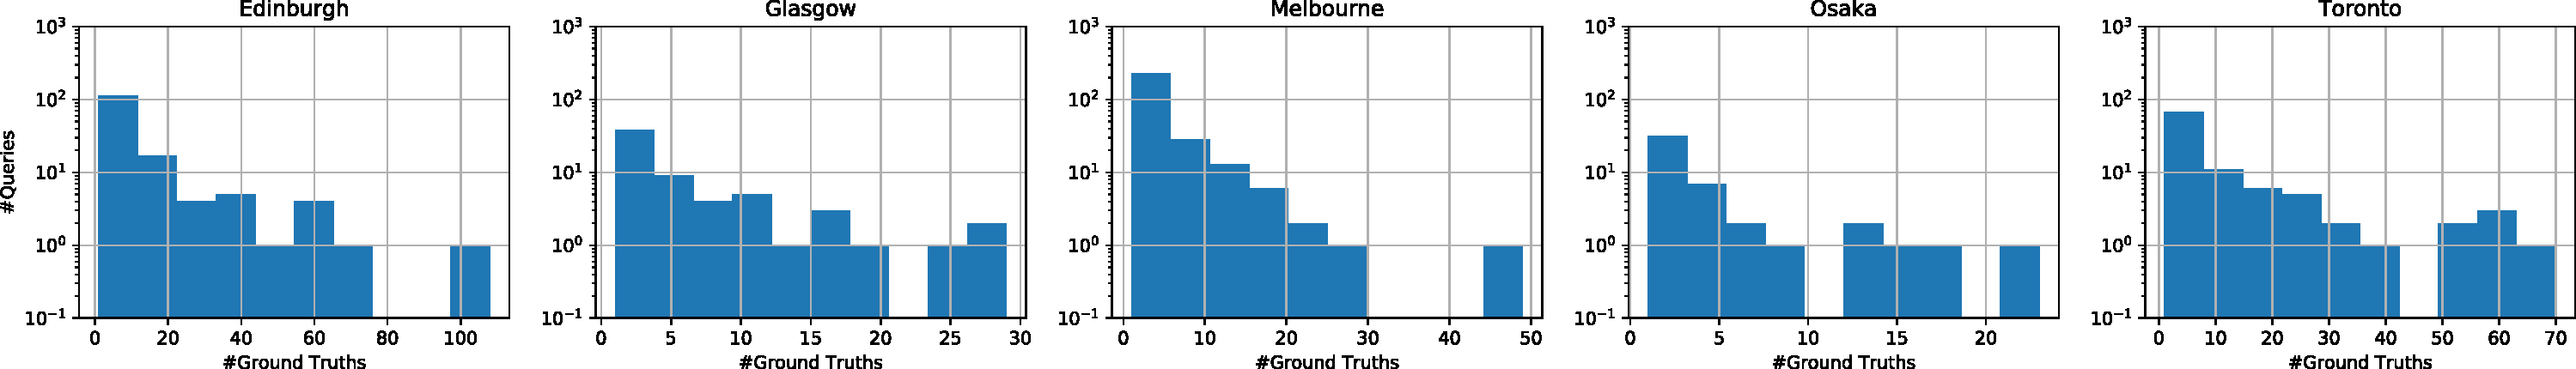
\includegraphics[width=\columnwidth]{hist.pdf}
	\caption{Histograms of the number of trajectories per query.}
	\label{fig:hist}
\end{figure}


\secmoveup
\subsection{Methods compared}
\textmoveup

We compare the performance of our methods to the following three baselines:
\begin{itemize}[leftmargin=0.125in]\itemmoveup
\parskip -.05em
	\item The \textsc{Random} baseline simply recommends a sequence of POIs by sampling uniformly at random from the whole set of POIs (without replacement).

	\item The stronger \textsc{Popularity} baseline recommends the top-$k$ most popular POIs i.e. the POIs that have been visited the most in the training set.

	\item \textsc{PoiRank}~\cite{cikm16paper} is a generalisation of \textsc{Popularity} which considers a number of POI features in addition to the popularity,
and trains a RankSVM model to learn a score for each POI. The top-$k$ scoring POIs are then used to construct a trajectory.
\end{itemize}\itemmoveup

To assess the viability of our structured prediction approach, and the necessity of our two extensions (normalising the loss per query and disallowing loops), we implemented the following versions of our structured prediction methods.
All variants predicts with the list Viterbi algorithm (Section~\ref{ssec:subtour}) to generate a path.
\begin{itemize}[leftmargin=0.125in]\itemmoveup
\parskip -.05em
	\item The structured prediction ({\sc SP}) method employs the vanilla structured SVM framework in order to learn a score for trajectories given a query.

	\item The structured recommendation ({\sc SR}) method extends the {\sc SP} method by additionally incorporating multiple ground truths into
	forming the constraints and adding them in cutting-plane algorithm,
	described in Section~\ref{ssec:sr} and \ref{ssec:SRinf}.
	%performing normalisation of the loss function per query,
	%so that we do not attempt to distinguish between multiple ground truths for the same query.

	\item The variants {\sc SPpath} and {\sc SRpath} extend the above methods by enforcing the constraint during training that sequences with loops are disallowed.
\end{itemize}\itemmoveup


\secmoveup
\subsection{Evaluation procedure}
\textmoveup

% leave-one-out evaluation (with query aggregation)
%As described in Section~\ref{sec:queryagg},
%To evaluate the performance of the various methods under comparison,
%we first group the trajectories  %according to queries that they conform to.
We then evaluate the performance of each algorithm using leave-one-query-out cross validation. That is, holding out each query $\x\pb{i}$, and also all of its relevant trajectories $\{\y\pb{ij}\}_{j=1}^{n^i}$ in each round.
where in each iteration of this procedure,
%one query and its associated trajectories serves as a test point, with all other trajectories for training.
%(Note that without this query aggregation, there will be considerable overlap between the train and test set, and simple nearest neighbour methods will be hard to outperform.)
% model selection (Monte Carlo CV) (with query aggregation): 90/10 random split for 5 times
Relevant hyper-parameters (e.g.\ the regularisation constant $C$) are tuned using Monte Carlo cross validation~\cite{burman1989comparative} on the training set.

We use three different measures to compare algorithm performances.
The {\bf F$_1$ score on points}~\cite{ijcai15} computes F$_1$ on the predicted versus seen points
without considering their relative order.
The {\bf F$_1$ score on pairs}~\cite{cikm16paper} is proposed to mitigate this by computing F$_1$ on all ordered pairs in the predicted versus groundtruth sequence. It is 1 iff both sequences agree completely.
The well-known rank correlation {\bf Kendall's $\tau$} (version $b$)~\cite{agresti2010analysis} computes the ratio of concordant (correctly ranked) pairs minus discordant pairs, over all ($\frac{1}{2}l(l-1)$) pairs.
\eat{
% evaluation metric: kendall's Tau (mention F1, pF1)
We use three performance measures to assess the test fold performance of each algorithm:
point-F$_1$ score~\cite{ijcai15},
pairs-F$_1$ score~\cite{cikm16paper},
and
Kendall's $\tau$ (version $b$)~\cite{kendall1945,agresti2010analysis}.
\TODO{explain point and pairs}

Kendall's $\tau$
essentially measures the fraction of pairs of POIs that are correctly ordered in the prediction and ground truth sequences,
with adjustment for ties.
In particular,
define the rank of POIs $\mathcal{P}$ in a trajectory $\mathbf{y} = (y_1,\dots,y_K)$ as
the position of the POI within the trajectory,
\begin{align*}
r_\mathbf{y} &= (r_1,\dots,r_j,\dots,r_{|\mathcal{P}|}), \\
r_j &= \sum_{k=1}^K (| \mathcal{P} | - k + 1)  \llb p_j = y_k \rrb, ~ j = 1, \dots, | \mathcal{P} |.
\end{align*}
The Kendall's $\tau$ score is then computed on $r_\mathbf{y}$ versus $r_\mathbf{\hat{y}}$.
Unlike the F$_1$ scores on points and pairs,
which only care about the set of correctly recommended POIs or POI pairs,
this metric taking both factors into account.
}

Structured recommendation problems aims to perform ranking on a very large $m^l$ labelset.
We adopt the practice of {\em best of top 10}~\cite{russakovsky2015imagenet} for reporting results. Or, predict top 10 trajectories and then report the best match of any in the top 10 to any trajectory in the ground truth set.
\eat{
As described previously, our methods are capable of recommending not merely a single trajectory,
but rather a list of trajectories.
While one can simply take the top recommended trajectory as the prediction,
this ignores the fact that there are likely multiple plausible trajectories for any given query.
Thus, for each performance measure $\mathrm{perf}$,
we take the maximum over all trajectories,
i.e.,
\begin{equation*}
%\tau_b^{(i)} =
\mathrm{perf}^{(i)}( \mathbf{y}, \hat{\mathbf{y}} ) =
\max_{(\mathbf{y}, \hat{\mathbf{y}}) \in \{\mathbf{y}^{(ij)}\}_{j=1}^{N_i} \times \{\hat{\mathbf{y}}^{(ij)}\}_{j=1}^k}
%\tau_b(r_\mathbf{y}, r_{\hat{\mathbf{y}}}),
\mathrm{perf}(\mathbf{y}, {\hat{\mathbf{y}}}),
\end{equation*}
where $\{\mathbf{y}^{(ij)}\}_{j=1}^{N_i}$ are the ground truths for query $\mathbf{x}^{(i)}$ and
$\{\hat{\mathbf{y}}^{(ij)}\}_{j=1}^k$ are the top-$k$ recommendations.
}

\secmoveup
\subsection{Results and discussion}
\label{sec:result}
\textmoveup

% !TEX root = ./main.tex

\begin{table*}[t]
\caption{Experimental results on trajectory recommendation datasets. The top three rows are baselines, and the bottom four are the methods proposed in this paper. Bolded entries correspond to the best performing method for each metric; italicised entries to the next best method. Higher scores are better.}
\label{tab:result}
\centering
%\setlength{\tabcolsep}{3pt} % tweak the space between columns
\small
\begin{tabular}{l|cc|cc|cc} \hline
                    & \multicolumn{2}{|c}{\textbf{Kendall's $\tau$}}
                    & \multicolumn{2}{|c}{\textbf{F$_1$ score on points}}
                    & \multicolumn{2}{|c}{\textbf{F$_1$ score on pairs}} \\ \cline{2-7}
                    & Osaka & Glasgow 
                    & Osaka & Glasgow  
                    & Osaka & Glasgow \\ \hline
\textsc{Random}     & $0.403\pm0.025$ & $0.410\pm0.032$  
                    & $0.430\pm0.021$ & $0.451\pm0.027$  
                    & $0.057\pm0.024$ & $0.136\pm0.037$ \\
\textsc{Popularity} & $0.567\pm0.034$ & $0.646\pm0.035$  
                    & $0.601\pm0.031$ & $0.681\pm0.032$  
                    & $0.277\pm0.051$ & $0.416\pm0.050$ \\
\textsc{PoiRank}    & $0.646\pm0.040$ & $0.736\pm0.030$  
                    & $0.678\pm0.037$ & $0.764\pm0.027$  
                    & $0.425\pm0.058$ & $0.550\pm0.047$ \\
\midrule
\textsc{SP}         & $0.796\pm0.037$ & $0.865\pm0.027$  
                    & $0.817\pm0.034$ & $0.878\pm0.024$  
                    & $0.665\pm0.055$ & $0.772\pm0.040$ \\
\textsc{SPpath}     & $0.794\pm0.035$ & $0.740\pm0.034$  
                    & $0.814\pm0.032$ & $0.764\pm0.030$  
                    & $0.653\pm0.054$ & $0.591\pm0.047$ \\
\textsc{SR}         & $\mathbf{0.814\pm0.034}$ & $\mathit{0.870\pm0.025}$  
                    & $\mathbf{0.832\pm0.031}$ & $\mathit{0.887\pm0.022}$ 
                    & $\mathit{0.673\pm0.053}$ & $\mathit{0.774\pm0.039}$ \\
\textsc{SRpath}     & $\mathit{0.805\pm0.036}$ & $\mathbf{0.877\pm0.025}$ 
                    & $\mathit{0.821\pm0.033}$ & $\mathbf{0.893\pm0.021}$ 
                    & $\mathbf{0.682\pm0.054}$ & $\mathbf{0.792\pm0.038}$ \\ \hline
\end{tabular}
\end{table*}


% experimental results
The performance of three baselines and four variants based on structured prediction on two datasets are shown in Table~\ref{tab:result}.
From these results, we can make the following key inferences that validate our contributions.

\textbf{Exploiting the structure of sequences helps}.
We find that all variants of our structured prediction methods achieve better performance than existing baselines.
This indicates that the basis of our approach -- reducing sequence recommendation to a structured prediction problem -- is sensible, and has empirical benefit.

\textbf{Accounting for multiple ground truths helps}.
We find that \textsc{SR} always performs better than \textsc{SP},
and similarly for the {\sc path} variants of both methods.
This indicates that our first extension -- explicitly modelling multiple ground truths helps recommendation -- is important to achieve good performance.
(We note that even without this correction, our structured methods outperform baselines.)

\textbf{Eliminating loops during training helps}.
We find that {\sc SRpath} improves performance further of the {\sc SR} method,
as indicated by the F$_1$ score on pairs.
This indicates that our second extension -- explicitly performing sub-tour elimination in training -- is important to further improve performance.
Interestingly,
this advantage does \emph{not} take effect if the multiple ground truths are not modelled explicitly,
with the performance of the {\sc SP} method largely unaffected.

\textbf{An illustrative example}. Figure~\ref{fig:example} consist of an example that illustrates the difference among the different algorithm variants. The query requires the trajectory to start from the middle point and be of length 2.
\textsc{PoiRank} regards points at the lower right and upper left be of the highest rank, but did not consider their compatibility (\ie pairwise features). {\sc SP} and {\sc SR} hits one edge out of the two the groundtruth (green edge), while {\sc SRpath} hits both edges for two valid trajectories after taking all factors into account.

Overall, these results indicate that our structured prediction approach to the problem has
benefits over non-structured approaches,
and that our extensions to the vanilla structured approach are important to further improve performance.

%\subsection{Example}
%\label{sec:example}

\begin{figure*}[t]
	\centering
	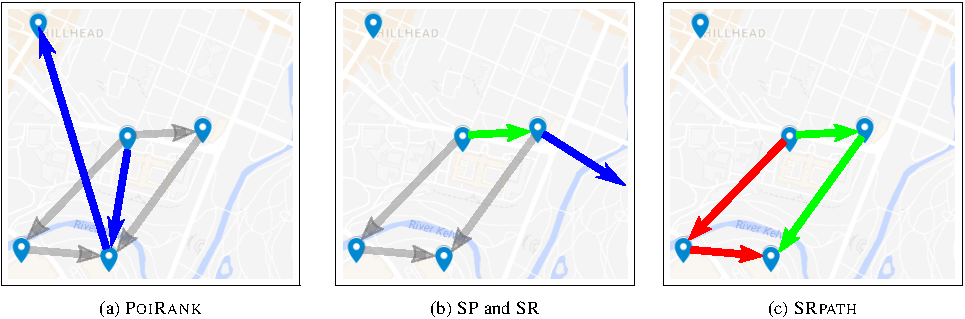
\includegraphics[width=0.9\textwidth]{example.pdf}
	\caption{Example of structured recommender versus baseline on a query with two ground truths as shown in Figure (c).
             (a) \textsc{PoiRank} cannot make a recommendation related to any of the ground truths;
             (b) \textsc{SP} and \textsc{SR} recommend a better trajectory than \textsc{PoiRank}, but not fully consistent with the ground truths;
             (c) \textsc{SRpath} hit both ground truths at rank 3 and 5 respectively.}
	\label{fig:example}
\end{figure*}



\bibliographystyle{ieeetr}
\bibliography{ref}

\end{document}
